\documentclass[11pt]{article}
\usepackage[margin=1in]{geometry}
\usepackage{booktabs,multirow,amsmath,amssymb,graphicx,xcolor,url}
\usepackage[numbers,sort&compress]{natbib}
\usepackage{hyperref}

\title{How Fragile Is Your Vocabulary? A Controlled Audit of\\
Inference-Vocabulary Robustness in Training-free\\
Open-Vocabulary Semantic Segmentation}
\author{Thomas Sam\thanks{Author list and affiliations to be finalized before arXiv submission.}}
\date{July 30, 2026}

\newcommand{\miou}{mIoU}

\begin{document}
\maketitle

\begin{abstract}
Training-free open-vocabulary semantic segmentation (OVSS) is evaluated as if the
inference vocabulary were a fixed, clean, given input, yet the promise of the task is
precisely that users supply arbitrary class names at test time. We present a controlled
audit of inference-vocabulary robustness. We freeze a single inference protocol and
perturb only the vocabulary along three orthogonal axes---synonym substitution,
granularity shift, and distractor injection---across three representative training-free
methods (MaskCLIP, SCLIP, ClearCLIP; key cells replicated on NACLIP) and four
benchmarks (VOC-21, COCO-171, ADE-150, PC-459); the core audit matrix comprises
about 150 evaluation runs, and the full study archives over 600. The audit yields five findings.
(1) Undocumented class-name engineering in official vocabularies is worth
11.8--20.6 \miou{} on VOC-21 across the three main-matrix methods (up to 22.1 on
the extended seven-method leaderboard), comparable to or exceeding the
gaps between methods.
(2) WordNet-filtered synonym substitution costs up to 6 \miou{} on the three
main-matrix methods (up to 7 in the replication and backbone checks), with a 3.7 \miou{}
spread across random substitution seeds, and one-level hypernym substitution halves
VOC-21 and nearly zeroes ADE-150 performance.
(3) Injecting distractor classes \emph{raises} \miou{} over ground-truth classes by up
to 10 points while lowering an object-crop classification control by 18.5 points; the
gain reverses into a drop once the engineered background vocabulary is used, isolating
background under-modelling as the mechanism and showing that dense vocabulary
sensitivity cannot be read off classification behaviour.
(4) Pre-registered text-side repairs (mean-centering, vocabulary-conditioned and global
ZCA whitening) improve embedding-space separability metrics monotonically yet reduce
\miou{} in 8 of 9 method$\times$dataset cells on mid-to-large vocabularies, showing
that text embedding geometry is not a reliable proxy for segmentation quality.
(5) A constructive attempt to automate vocabulary engineering recovers most of its
macro-\miou{} value (up to $+18.8$ on plain vocabularies) with synthesised background
negatives, but every pre-registered label-free mechanism for its per-class protective
component fails, indicating engineered vocabularies encode supervision that text-side
machinery cannot reconstruct. We release the perturbation protocol, vocabularies, and
evaluation harness to make vocabulary robustness a reportable, comparable quantity.
\end{abstract}

\section{Introduction}

Open-vocabulary semantic segmentation promises segmentation for class sets specified
freely at inference time. A rapidly growing family of \emph{training-free} methods
\citep{zhou2022maskclip,wang2024sclip,lan2024clearclip,hajimiri2024naclip,lan2024proxyclip}
adapts CLIP \citep{radford2021clip} to dense prediction without any segmentation
training, and is evaluated by zero-shot \miou{} on standard benchmarks. In every such
evaluation, the inference vocabulary---the list of class names presented to the text
encoder---is treated as a fixed part of the benchmark. The open half of
``open-vocabulary'' is never itself tested.

This gap matters because the vocabulary is the only input the user controls. If
performance and method rankings change materially under semantically equivalent or
mildly perturbed vocabularies, then reported numbers measure a particular prompt
engineering artifact rather than open-vocabulary capability. Anecdotal evidence already
exists: public implementations ship hand-tuned class-name files (e.g.\ expanding the
VOC ``background'' class into 26 scene sub-classes \citep{wang2024sclip}), and prompt
augmentation methods \citep{roth2023waffle,pratt2023cupl} show that name phrasing shifts
classification accuracy. What is missing is a controlled, dense-prediction-specific
audit that isolates the vocabulary as the sole experimental variable.

We provide such an audit. We freeze one inference protocol---backbone, templates,
resolution, sliding window, logit pooling---and vary only the vocabulary along three
orthogonal axes: (i) \emph{synonym substitution} with WordNet+CLIP-similarity filtering
at 25/50/100\% replacement rates and three seeds; (ii) \emph{granularity shift} via a
frozen first-sense WordNet hypernym rule; (iii) \emph{distractor injection} of 50--200
out-of-dataset class names stratified by text similarity. We evaluate three
representative training-free methods on four benchmarks spanning 21 to 459 classes:
VOC-21 \citep{everingham2010voc}, COCO-171 \citep{lin2014coco,caesar2018cocostuff},
ADE-150 \citep{zhou2017ade}, and PC-459 \citep{mottaghi2014context}.
Alongside the audit we pre-registered two text-side repair hypotheses with kill
criteria: vocabulary-conditioned whitening of class embeddings, and its comparison
against global-statistics whitening. KC1 failed outright; KC2's literal criterion is
met only on COCO-171, where both whitening variants remain well below the unwhitened
baseline, so no usable repair emerges. We report these failures as findings.

Our contributions are:
\begin{enumerate}
\item \textbf{A frozen three-axis vocabulary perturbation protocol} for OVSS, with
  released perturbed vocabularies, exclusion rules for non-semantic classes, and a
  uniform inference protocol that removes per-method prompt engineering.
\item \textbf{An audit of three training-free methods on four benchmarks} showing that
  (a) undocumented name engineering is worth 11.8--20.6 \miou{} (up to 22.1 on the
  extended leaderboard of Table~\ref{tab:robustbench}), comparable to or larger
  than method-to-method gaps; (b) synonym-seed spread reaches 3.7 \miou{}, larger than
  many reported improvements; (c) the relative ordering of methods is not stable across
  vocabulary regimes (e.g.\ ClearCLIP leads SCLIP by 2.5 \miou{} on PC-459 while
  trailing by 1.8 under the official VOC-21 vocabulary).
\item \textbf{Dense-specific evidence}: under distractor injection, an object-crop
  classification control drops by 18.5 points while segmentation \miou{} \emph{rises}
  by up to 10 points---and the gain reverses under the engineered background
  vocabulary---exposing a background-absorption pathology of the \miou{} protocol;
  vocabulary robustness conclusions cannot be imported from classification.
\item \textbf{A negative result on text-side repair}: mean-centering and ZCA whitening
  (vocabulary-conditioned or global; verdict pre-registered at shrinkage 0.5 and
  confirmed by a post-verdict shrinkage sweep) improve embedding margin and effective
  rank monotonically yet decrease \miou{} in 8 of 9 mid-to-large-vocabulary
  cells---embedding-geometry diagnostics are not a proxy for segmentation quality.
\item \textbf{A constructive decomposition of vocabulary engineering}
  (\S\ref{sec:vabs}): its macro-\miou{} value is largely an automatable
  background-sink effect (synthesised negatives recover $+16.1$ macro on VOC-21
  plain vocabularies without harming official ones), while its per-class protective
  component resisted every pre-registered label-free mechanism (three signal
families in the main text; seven entries in the appendix index), isolating exactly
  where label-derived knowledge enters current benchmarks.
\end{enumerate}

\section{Related Work}

\paragraph{Training-free OVSS.} Open-vocabulary segmentation was first pursued with
training: language-aligned decoders and mask classifiers fine-tuned on segmentation or
image-text data \citep{li2022lseg,ghiasi2022openseg,xu2022groupvit,liang2023ovseg,xu2023san,cho2024catseg},
or learned from image-text pairs alone \citep{shin2022reco,cha2023tcl}. The
training-free line instead re-reads a frozen CLIP \citep{radford2021clip}:
MaskCLIP \citep{zhou2022maskclip} extracts dense
predictions from CLIP by converting the final attention pooling into a value-only
pathway; SCLIP \citep{wang2024sclip} uses correlative self-attention
($\mathrm{softmax}(qq^\top)+\mathrm{softmax}(kk^\top)$); ClearCLIP
\citep{lan2024clearclip} additionally drops the residual path and FFN; NACLIP
\citep{hajimiri2024naclip} enforces neighbourhood-aware attention via a Gaussian
spatial prior; ProxyCLIP \citep{lan2024proxyclip} imports affinities from visual
foundation models; GEM \citep{bousselham2024gem} and CLIP-DINOiser
\citep{wysoczanska2024clipdinoiser} are further representatives. All are evaluated on
fixed official vocabularies; none reports vocabulary sensitivity. We audit MaskCLIP,
SCLIP, and ClearCLIP as representative final-block variants under one protocol, and
scope our conclusions to this family (\S\ref{sec:limitations}).

\paragraph{Text-side sensitivity and name quality.} On the classification side, prompt
template ensembles \citep{radford2021clip}, learned soft prompts \citep{zhou2022coop},
LLM-generated descriptions
\citep{pratt2023cupl}, random descriptors \citep{roth2023waffle}, WordNet-hierarchy
augmentation \citep{ge2023hierarchy}, concept-frequency analyses
\citep{parashar2024neglected}, and synonym-space aggregation \citep{yin2026s3} all show
that name phrasing shifts zero-shot accuracy; vocabulary-free classification
\citep{conti2023vocabularyfree} questions the given-vocabulary assumption itself. For
segmentation, RENOVATE \citep{huang2024renovating} shows benchmark class names are
often misaligned with masks and that \emph{renaming} them changes results
substantially, and FLOSS \citep{benigmim2025floss} shows per-class template selection
alone improves a frozen segmenter; SynCLIP \citep{wang2026synclip}
confirms synonym-induced grounding inconsistency in dense perception and
repairs it by synonym-coherent \emph{re-pretraining} --- adapting the model
to the names, whereas we freeze the model and perturb the names, so our
protocol can audit SynCLIP-class models directly. A data-centric retrieval
family (ReME~\citep{xuan2025reme}) replaces attention surgery with
reference-set retrieval; its released repository contains no method code
at audit time, so it is not among our anchors, but its name-mediated retrieval
interface makes it a natural future audit subject. A training-free class-purification
plugin (FreeCP~\citep{freecp2025}) manipulates the query set itself, making
it a natural interlocutor for our distractor axis; however, its released
code, in its official configuration (the LLM dictionaries are consumed
unconditionally inside its purification step, with no non-LLM mode), requires
precomputed per-name LLM (Vicuna-13B) description
dictionaries keyed to the official engineered class names, so at audit time a plain,
synonym, or distractor vocabulary cannot even be expressed without
regenerating those assets --- vocabulary engineering one level deeper than
the class-name files we perturb --- and it therefore cannot be audited
under our only-change-the-name-files protocol. We differ on both axes of intent: these works
\emph{improve} names or prompts toward a better fixed evaluation, whereas we hold
labels fixed and \emph{measure the response} of methods to controlled, user-plausible
vocabulary perturbations---including axes (distractor injection, granularity, seed
variance of synonym choice) that name-improvement work does not quantify---plus
pre-registered tests showing that generic whitening-style repairs do not transfer to
dense prediction.

\paragraph{Background modelling in OVSS.} That an explicit background model matters
is folklore in the method literature: CaR \citep{sun2024car} adds hand-written
background queries, OVDiff \citep{karazija2024ovdiff} derives negative visual
prototypes from a diffusion model, and SCLIP's official VOC vocabulary expands
``background'' into 26 scene sub-classes \citep{wang2024sclip}. Our constructive
experiment (\S\ref{sec:vabs}) differs in intent from these methods: rather than
proposing another background mechanism, it uses pre-registered text-side background
synthesis---with random-word controls and per-class safety criteria---to decompose
\emph{how much} of the engineered-vocabulary value such mechanisms can recover
without labels, and which component cannot.

\paragraph{Embedding geometry.} CLIP text embeddings concentrate in a narrow cone;
for sentence embeddings, whitening improves STS performance and speeds up retrieval
via dimensionality reduction \citep{su2021whitening}. We confirm the cone
(mean pairwise cosine 0.77--0.82 across vocabularies) and show that removing it helps
linear separability metrics but not segmentation, a dissociation previously unreported.

\paragraph{Evaluation audits and metrics.} MESS \citep{blumenstiel2023mess} audits
zero-shot segmentation across \emph{domains}; our audit varies the complementary input,
the vocabulary. \citet{zhou2023rethinking} show pixel-wise IoU mishandles
synonym/near-synonym predictions and propose Open mIoU, and \citet{huang2025revisit}
study vocabulary expansion with semantically ambiguous words and propose a mask-wise
protocol; our distractor results (\S\ref{sec:distractor}) explain when expansion
raises rather than lowers the reported number---the direction is governed by
background modelling and metric convention---and support adopting such open-set-aware
metrics. A concurrent ``systematic audit'' of VLM robustness to natural
semantic variation \citep{beyondbench2026} targets classification/retrieval
under typographic and semantic variants, not dense segmentation or
inference-vocabulary perturbation. In remote sensing, the concurrent
OVEarth-Bench \citep{li2026ovearthbench} scores open-vocabulary Earth-observation
models on category breadth and query diversity within a fixed benchmark
vocabulary (negatives are absent classes to be rejected); it does not perturb
the names of a fixed target class, which is the axis audited here. Our motivation
parallels the classification test-set audits that asked whether reported gains
survive a change of the nominally-fixed evaluation input
\citep{recht2019imagenetv2,beyer2020imagenet}: there the images, here the names. To our knowledge no prior work performs a controlled multi-axis
inference-vocabulary perturbation audit across training-free OVSS methods; the closest
works study name quality \citep{huang2024renovating} or template choice
\citep{benigmim2025floss} in isolation. Together these lines form three
orthogonal axes of open-vocabulary evaluation --- open-set-aware scoring
functions \citep{zhou2023rethinking}, static class-name quality
\citep{huang2024renovating}, and (here) dynamic perturbation of the
inference vocabulary itself; progress on one axis does not substitute for the
others. Our protocol is designed to be re-runnable on
future methods.

\section{Audit Protocol}
\label{sec:protocol}

\paragraph{Frozen inference protocol.} OpenCLIP \citep{ilharco2021openclip} ViT-B/16
(OpenAI weights, QuickGELU); the 80 ImageNet prompt templates
\citep{radford2021clip}; short side 336, sliding window 224, stride 112, mean
logit fusion; temperature 40 softmax over sub-queries followed by per-class max pooling
(the convention of \citet{wang2024sclip}); identical for all methods and conditions.
\miou{} is computed over classes present in ground truth. No PAMR
\citep{araslanov2020pamr} or other post-processing. Under this protocol our SCLIP reproduction reaches 55.4 \miou{} on
VOC-21 with the official class-name file (paper: 59.1 with additional refinement),
which we consider adequate for controlled comparisons since all conditions share the
identical pipeline. Throughout the paper, differences and deltas quoted in the text
are computed from unrounded run records; they may differ from differences of the
displayed values (rounded to 0.1) by up to 0.1.

\paragraph{Axis 1: synonym substitution.} For each class, candidate synonyms are
WordNet \citep{miller1995wordnet} noun-synset lemmas filtered by CLIP text cosine similarity to the original name
within $[0.70, 0.95]$; the highest-similarity candidate is chosen. Classes without
valid candidates, and non-semantic classes (\texttt{background}, \texttt{unknown},
\texttt{other}), are never substituted. We replace 25/50/100\% of substitutable classes
with three random seeds at 50\%. Ground-truth labels are unchanged.

\paragraph{Axis 2: granularity shift.} Each class name is replaced by the first lemma
of the first-sense direct WordNet hypernym (frozen rule, no manual correction), with the
same exclusion list. The mapping table is part of the released protocol
(Appendix~\ref{app:artifacts}); merged-credit scoring (crediting predictions of a
coarse name shared by several classes) is left to future work.

\paragraph{Axis 3: distractor injection.} Distractors are drawn from the union of
ADE-847 and PC-459 vocabularies minus the target vocabulary, filtered to CLIP text
cosine $\le 0.92$ against all target classes (synonym guard), stratified into
\emph{near} ($>0.80$), \emph{mid} ($0.65$--$0.80$) strata, and injected at $+50$ and
$+200$. Predictions of distractor classes count as errors for the ground-truth class.

\paragraph{Pre-registered repair hypotheses.} Before running segmentation experiments
we froze two kill criteria: (KC1) vocabulary-conditioned ZCA whitening of class
embeddings must gain $>0.5$ \miou{} on large-vocabulary benchmarks across three
methods; (KC2) vocabulary-conditioned statistics must beat global statistics in at
least one regime. The pre-registered verdict was taken at shrinkage $0.5$; a
post-verdict sensitivity sweep over $\{0.1,0.3,0.7,0.9\}$ (PC-459, ClearCLIP) confirmed
the conclusion is not a shrinkage artifact.

\section{Results}

\subsection{Naming conventions are worth more than method choice}
\label{sec:naming}

\begin{table}[t]
\centering\small
\caption{VOC-21 (300 images). Official SCLIP vocabulary (background expanded to 26
sub-classes; synonym-enriched \texttt{person}/\texttt{tv}) vs.\ plain dataset names,
identical protocol. The naming convention is worth 11.8--20.6 \miou{}, comparable to
or larger than the method gaps.}
\label{tab:naming}
\begin{tabular}{lccc}
\toprule
Vocabulary & SCLIP & ClearCLIP & MaskCLIP \\
\midrule
Official (engineered) & \textbf{55.4} & 53.6 & 43.6 \\
Plain dataset names   & 34.8 & \textbf{34.9} & 31.8 \\
\midrule
$\Delta$ & $-20.6$ & $-18.7$ & $-11.8$ \\
\bottomrule
\end{tabular}
\end{table}

\begin{figure}[t]
\centering
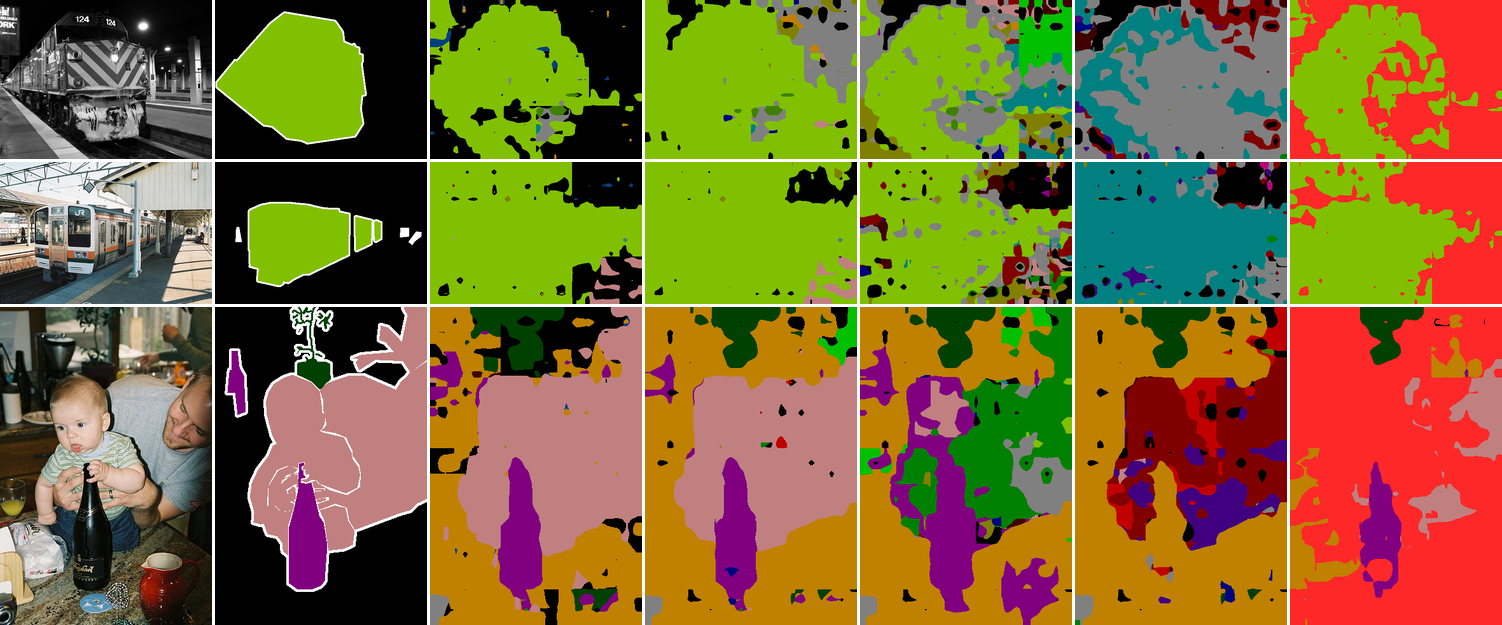
\includegraphics[width=\linewidth]{figs/fig_qual.png}
\caption{The same frozen SCLIP pipeline under five vocabularies (VOC-21 val). Columns:
image, ground truth, official (engineered) names, plain dataset names, 100\% synonym
substitution, one-level WordNet hypernyms, plain $+200$ near distractors
(distractor-class predictions in red). Only the list of class names changes between
columns 3--7; every visible degradation is a vocabulary effect, not a model change.}
\label{fig:qual}
\end{figure}

Table~\ref{tab:naming} and Figure~\ref{fig:qual} show the single largest effect in the audit: replacing the
engineered class-name file shipped with public code by the plain dataset names costs
11.8--20.6 \miou{}. That class names matter in OVSS benchmarks was established by
RENOVATE \citep{huang2024renovating}, which \emph{renames} classes to better match
masks; the measurement here is complementary---it quantifies, under a frozen protocol,
how much of a reported training-free number is attributable to an undocumented name
file rather than to the method. The method ordering is also regime-dependent: SCLIP
leads ClearCLIP by 1.8 under the official file, the two are statistically tied under
plain names (34.8 vs.\ 34.9, within subset-resampling noise), and ClearCLIP leads by
2.5 on PC-459. Since papers rarely document these files, cross-paper comparisons of
training-free OVSS numbers largely compare vocabulary engineering, supporting the
pre-registered naming-engineering and provenance claims.

\subsection{Synonym and granularity axes}
\label{sec:synonyms}

\begin{table}[t]
\centering\small
\caption{VOC-21 audit matrix (300 images, plain-name baseline, \miou{}). Synonym
substitution at rate $r$ (seed 0; seeds 0/1/2 shown for 50\%); one-level WordNet
hypernym substitution (granularity). Labels are unchanged in all conditions.
Single-subset values; the image-resampling noise floor is 3.1 \miou{}
(Fig.~\ref{fig:variance}a), so differences below that are not interpreted.}
\label{tab:axes}
\begin{tabular}{lccc}
\toprule
Condition & SCLIP & ClearCLIP & MaskCLIP \\
\midrule
plain (baseline)      & 34.8 & 34.9 & 31.8 \\
syn 25\%              & 34.1 & 32.9 & 29.6 \\
syn 50\% (s0/s1/s2)   & 34.4/31.3/30.7 & 33.3/32.8/31.2 & 29.4/29.3/27.7 \\
syn 100\%             & 30.6 & 29.0 & 26.3 \\
hypernym (coarse)     & 17.0 & 17.0 & 16.9 \\
\bottomrule
\end{tabular}
\end{table}

\begin{figure}[t]
\centering
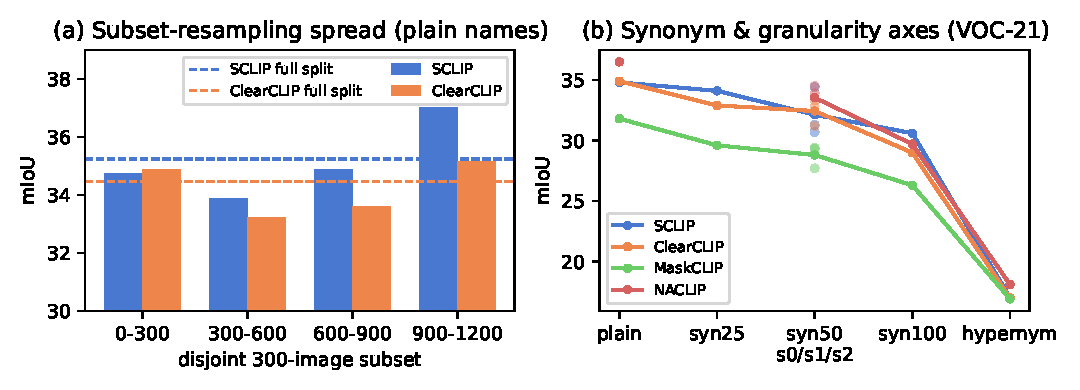
\includegraphics[width=\linewidth]{figs/fig_variance.pdf}
\caption{(a) Plain-name \miou{} on four disjoint 300-image VOC-21 subsets vs.\ the
full-split value (dashed): subset resampling alone spans up to 3.1 \miou{}, our noise
floor for method comparisons. (b) Synonym and granularity axes on VOC-21 for all four
methods; dots show the three 50\%-substitution seeds evaluated on the identical image
subset.}
\label{fig:variance}
\end{figure}

Synonym substitution costs 4--6 \miou{} at full replacement, and the spread across three
substitution seeds at 50\% reaches 3.7 \miou{} (Table~\ref{tab:axes}); since all seeds
are evaluated on the same fixed image subset, this spread reflects vocabulary choice
alone, not image sampling (per-method mean$\pm$std across seeds:
SCLIP $32.1\pm2.0$, ClearCLIP $32.4\pm1.1$, MaskCLIP $28.8\pm1.0$); on ADE-150 the
one-level hypernym rule collapses performance from 13.1/14.7/10.2 to 2.5/3.8/1.9. Both
axes use frozen, released rules, so these are reproducible lower bounds on user-facing
robustness: a user who says \emph{cattle} instead of \emph{cow} or \emph{motorcycle}
instead of \emph{motorbike} is not misusing an open-vocabulary system.

\subsection{Distractor injection: \miou{} rises while classification falls}
\label{sec:distractor}

\begin{table}[t]
\centering\small
\caption{Distractor injection on VOC-21. Top: plain-name baseline; bottom: the same
$+200$ near distractors added to the \emph{engineered} official vocabulary (26
background sub-classes). \miou{} is over ground-truth classes; the rightmost column is
classification accuracy on ground-truth-box crops with the same vocabulary, templates,
and pooling.}
\label{tab:distractor}
\begin{tabular}{lccc|c}
\toprule
Condition & SCLIP & ClearCLIP & MaskCLIP & Cls.\ acc.\ (SCLIP enc.) \\
\midrule
plain              & 34.8 & 34.9 & 31.8 & 72.8 \\
+50 near           & 42.3 & 39.3 & 36.9 & --   \\
+200 near          & 44.5 & 40.9 & 37.1 & 54.3 \\
+50 mid            & 41.5 & 38.2 & 36.0 & --   \\
\midrule
official           & 55.4 & 53.6 & 43.6 & -- \\
official +200 near & 52.5 & 51.6 & 41.9 & -- \\
\bottomrule
\end{tabular}
\end{table}

\begin{figure}[t]
\centering
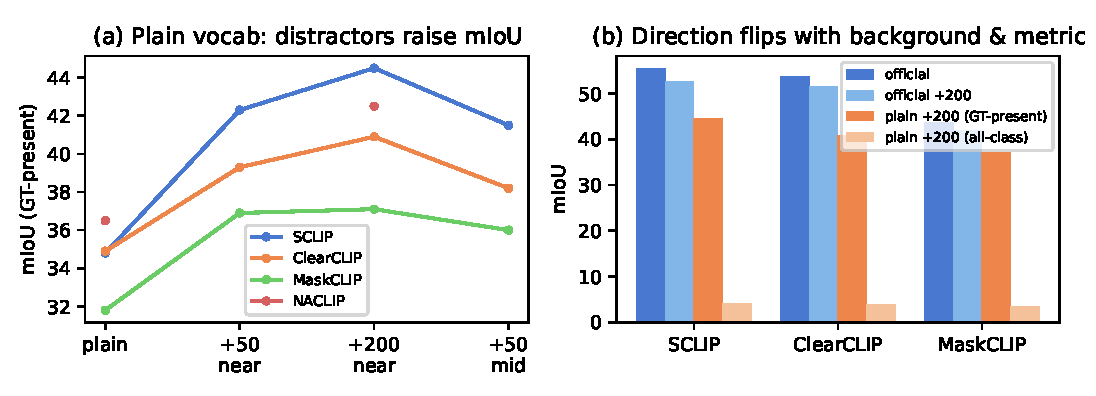
\includegraphics[width=\linewidth]{figs/fig_distractor.pdf}
\caption{(a) Adding distractors to the plain vocabulary \emph{raises} \miou{} over
ground-truth classes for all four methods. (b) The direction of the effect flips with
background modelling and metric convention: on the engineered official vocabulary the
same $+200$ distractors \emph{lower} \miou{}, and under the standard all-class \miou{}
the $+200$ condition collapses to $\sim$4.}
\label{fig:distractor}
\end{figure}

Injecting 200 near-domain distractor names \emph{raises} \miou{} by 5--10 points
(Table~\ref{tab:distractor}) while dropping matched classification accuracy by 18.5
points (single control cell: SCLIP encoder, VOC-21, $+200$ near; ground-truth-box
crops largely exclude background pixels, so this control shows the ranking behaviour
of an object-centric protocol rather than an exactly matched task). The mechanism of
the segmentation-side gain is background absorption: the plain \texttt{background} text
embedding fails to capture background pixels, so distractor classes absorb false
positives and boost the precision of ground-truth classes; \miou{} over ground-truth
classes then improves although every distractor prediction is an error. Two controls
support the mechanism. First, when the same $+200$ distractors are added to the
\emph{engineered} official vocabulary---whose 26 background sub-classes already absorb
background pixels---the gain reverses into a $1.7$--$2.9$ point \emph{drop}
(Table~\ref{tab:distractor}, bottom): the anomalous gain exists only where background
is under-modelled; once background is well modelled, vocabulary expansion behaves as
expected and hurts. Second, under the standard all-class \miou{}
(distractor classes entering the average with IoU $0$), the $+200$ near condition
collapses to $\sim$4 \miou{}: the direction of the vocabulary-expansion effect is
itself a metric choice. A pre-registered control re-draws the 200 near
distractors twice at random from the same frozen stratum (SCLIP/NACLIP,
test-300): the all-class collapse is stable across draws (spread
$\le$0.4 \miou{}), while the GT-present level varies by up to $\sim$4 \miou{}
(the deterministic first-200 draw is the harshest), so we treat the collapse as
draw-independent and quote GT-present magnitudes to that tolerance. This also reconciles our result with reports that vocabulary
expansion \emph{hurts} \citep{huang2025revisit}: with a well-modelled background or an
all-class metric, expansion hurts as expected; the anomalous gain appears exactly in
the common configuration---plain background name, \miou{} over ground-truth
classes---used by public training-free evaluations. A confusion-flow
decomposition over all seven audited methods (Appendix~\ref{app:badecomp})
makes this quantitative: the all-class drop is entirely a change of metric
convention (ground-truth-present accuracy in fact rises), 64--72\% of
ground-truth pixel mass flows to the injected names --- 83--88\% of that flow
from the background row, but 29--43\% of \emph{foreground} mass is also
stolen, so absorption is the dominant, not the only, mechanism --- inter-class
confusion \emph{decreases}, and the synonym axis shows the opposite signature
(pure inter-class confusion, zero convention effect). A pre-registered
capstone probe closes the repair question from above: pruning the
vocabulary to the \emph{ground-truth-present} classes (a presence oracle
no filter can beat) leaves all-class \miou{} at $\sim$4 on all three
models tested --- with a fixed 221-class denominator, 200 never-predicted
classes contribute IoU~0, so the all-class figure is structurally capped
near $(21/221)\times$ceiling for any method \emph{including the oracle},
while its GT-present effect is small and mixed ($-1.0$ to $+6.5$). Scope:
this holds under the fixed-denominator convention (our harness averages
over all $K$ classes, counting never-present, never-predicted classes as
IoU~0); under a NaN-exclusion convention that drops $0/0$ classes --- as
some standard toolchains do --- oracle pruning would restore the
denominator to the present classes and the ``collapse'' would disappear.
The distractor collapse is thus unrepairable by presence-based vocabulary
filtering under the fixed-denominator convention not because presence is
unknowable but because the convention itself charges the denominator ---
which convention a toolchain uses silently decides whether expansion
``hurts''; the open problem is metric design, not presence estimation.
A pre-registered contamination curve makes the absorption side graded:
injecting as few as $10$ random absent names raises GT-present \miou{}
by $+6$ to $+9$ (SCLIP/NACLIP, saturating near $+9$ to $+12$ at $150$),
with random names absorbing \emph{more} than near-distractors --- the
anomalous ``expansion helps'' regime begins at the very first injected
name and is pool-dependent, so any two benchmarks with different
vocabulary compositions already sit at different points of this curve.
A pre-registered mechanism probe pins the absorption gain down as
\emph{background calibration in disguise}: meaningless pseudo-words
reproduce half the random-name gain and $92\%$ of filler-captured
pixels are ground-truth background, but a single scalar background-logit
boost ($+0.02$ in cosine units, no fillers at all) exceeds the full
$50$-name gain ($47.5$ vs $46.5$ on SCLIP) --- the anomalous expansion
gain measures background under-calibration, and any absorption or
negative-vocabulary claim should be benchmarked against this
one-parameter control.
A pre-registered check confirms the convention choice does not disturb
\emph{comparisons}: recomputing all seven methods under
fixed-denominator, NaN-exclusion, and GT-present conventions leaves
method-ranking Spearman at $1.0$ on every axis. Two distinct facts
should not be conflated here: the \emph{oracle-pruned} ceiling of
$\sim$4 is a convention product (NaN-exclusion would restore the
denominator and dissolve it), whereas the \emph{unpruned} collapse is
real model behaviour under every convention --- unpruned models fire
on distractor names, so those classes are never $0/0$ and NaN-exclusion
does not rescue them. The convention decides what a number means, not
which method wins. This shows, first, that vocabulary sensitivity of dense
prediction is qualitatively different from classification, and second, that
neither \miou{} convention faithfully measures open-vocabulary segmentation quality
under vocabulary expansion, supporting open-set-aware metrics
\citep{zhou2023rethinking}.

\subsection{Pre-registered repairs fail; geometry is not a proxy}
\label{sec:whitening}

\begin{table}[t]
\centering\small
\caption{Text-side repairs under the frozen protocol (\miou{}). ZCA uses shrinkage 0.5;
global statistics from the ADE-847$\cup$COCO-171 vocabulary. Whitening hurts in every
cell (KC1 fails); vocabulary-conditioning edges out global statistics only on
COCO-171, where both remain clearly below the unwhitened baseline.}
\label{tab:whitening}
\begin{tabular}{llcccc}
\toprule
Dataset & Method & none & center & ZCA (vocab) & ZCA (global) \\
\midrule
PC-459  & SCLIP     & 12.8 & \textbf{13.7} & 11.6 & 11.9 \\
        & ClearCLIP & \textbf{15.3} & 15.2 & 13.2 & 13.7 \\
        & MaskCLIP  & \textbf{9.6}  & 9.3  & 8.2  & 8.4 \\
ADE-150 & SCLIP     & \textbf{13.1} & 12.4 & 10.8 & 10.9 \\
        & ClearCLIP & \textbf{14.7} & 13.9 & 12.7 & 12.9 \\
        & MaskCLIP  & \textbf{10.2} & 9.2  & 8.1  & 8.3 \\
COCO-171& SCLIP     & \textbf{22.9} & 21.2 & 19.9 & 18.9 \\
        & ClearCLIP & \textbf{24.2} & 23.1 & 21.7 & 21.4 \\
        & MaskCLIP  & \textbf{17.4} & 15.5 & 15.2 & 14.4 \\
\bottomrule
\end{tabular}
\end{table}

\begin{figure}[t]
\centering
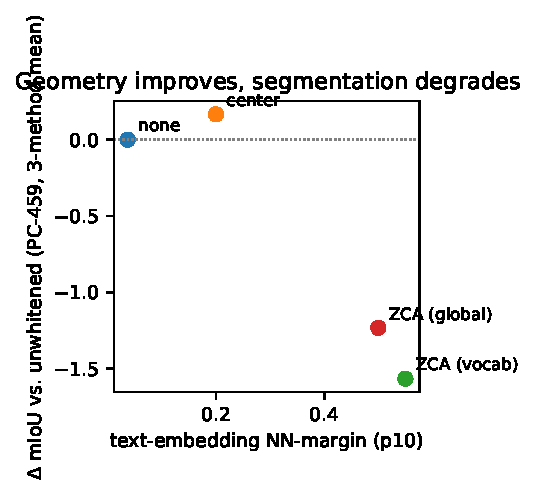
\includegraphics[width=0.55\linewidth]{figs/fig_decouple.pdf}
\caption{Text-side repairs on PC-459: each repair improves the embedding-space
nearest-neighbour margin (x-axis) yet changes segmentation \miou{} (y-axis,
three-method mean) by at most $+0.2$ (centering) and down to $-1.6$ (ZCA,
vocabulary-conditioned; largest single cell $-2.1$, ClearCLIP)---embedding
geometry is not a
proxy for dense segmentation quality.}
\label{fig:decouple}
\end{figure}

Raw class embeddings exhibit the expected cone geometry (mean pairwise cosine 0.77 on
A-847 to 0.82 on VOC-21; 10th-percentile nearest-neighbour margin shrinking from 0.078
to 0.037 as vocabularies grow), and ZCA whitening repairs every geometric diagnostic
(A-847 margin 0.09$\to$0.55, effective rank 154$\to$309). Yet Table~\ref{tab:whitening}
shows ZCA whitening \emph{reduces} \miou{} in all 9 method$\times$dataset cells and
centering in 8 of 9 (the exception: centering helps SCLIP on PC-459 by $+0.9$); the
post-verdict sensitivity sweep is monotone in shrinkage (PC-459/ClearCLIP: 11.6 at
$s{=}0.1$ up to 14.7 at $s{=}0.9$ vs.\ 15.3 unwhitened), and vocabulary-conditioned
statistics beat global ones only on COCO-171 (by 0.3--1.0), where both variants remain
2--4 points below the unwhitened baseline---so the conditioning advantage KC2 was
designed to detect never materialises as a usable repair. The only consistently
positive cases are
small-vocabulary VOC-21 ($+0.9$ to $+1.5$ for ZCA on the 300-image plain
split; archived in the artifact's run log, not tabulated in
Table~\ref{tab:whitening}, whose scope is the mid-to-large regime where the
verdict is taken). Two caveats bound the scope of
this negative result: whitening is applied to text queries only, against un-whitened
visual features, and we did not re-tune the logit temperature after whitening; joint
or temperature-recalibrated variants might behave differently. The dissociation claim,
however, needs only these cells: embedding separability improves monotonically while
dense transfer degrades, so geometry diagnostics alone cannot certify a text-side
repair.

\paragraph{Two further pre-registered failures.} Two later probes sharpen the
dissociation. (i) A frozen text-only vulnerability predictor (z-scored
nearest-neighbour margin plus semantic drift to the plain names) was tested
for ranking \emph{vocabularies} against the archived benchmark \miou{}
values: median per-method Spearman is 0.03 on the full VOC suite (kill
threshold 0.5) --- the same class of geometry signal that ranks surgery
\emph{configurations} at a fixed vocabulary with $\rho=0.89$
(Appendix~\ref{app:headlens}) carries no information across vocabularies at a
fixed configuration. (ii) A transductive prediction-space repair (RECAL:
name-conditioned additive logit debiasing toward a mass-flattening prior,
estimated label-free from the evaluation stream, frozen before the run)
reduces \miou{} in every cell (SCLIP plain $34.8\to27.6$, syn100
$30.6\to23.3$; NACLIP analogous): predicted class-mass imbalance under a
perturbed vocabulary is dominated, in this setup, by legitimate scene
statistics rather than name-conditional bias, so re-balancing it injects
more error than it removes (verdict scoped to the single frozen prior
strength $\alpha{=}0.5$; no post-verdict sweep was run).

\subsection{Can vocabulary engineering be automated? A constructive attempt}
\label{sec:vabs}

The audit's largest effect---the 12--21 point value of engineered vocabularies---raises
an obvious constructive question: can the engineering be synthesised automatically for
an arbitrary user vocabulary, training-free and text-side only? We pre-registered and
tested such a method (Vocabulary-Adaptive Background Synthesis, VABS): build a
candidate lexicon of scene/stuff words (COCO-Stuff\,$\cup$\,ADE-150 names), remove
candidates within cosine $\tau_{\mathrm{sim}}$ of any target class, greedily select
$M$ diverse negatives (facility-location objective), append them as sub-queries of the
background class, and fold their predictions into background. Hyper-parameters were
selected on a 100-image development set disjoint from the 300-image test set
($M{=}64$, $\tau_{\mathrm{sim}}{=}0.9$).

\begin{figure}[t]
\centering
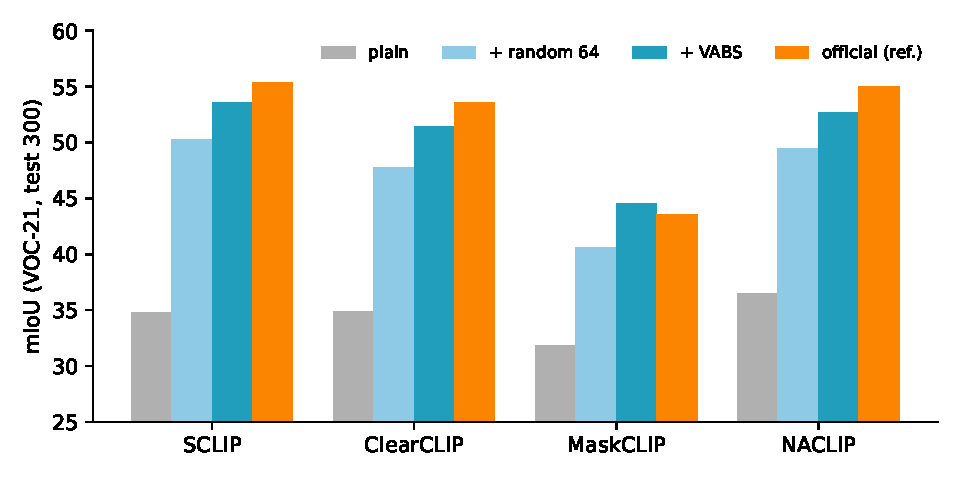
\includegraphics[width=0.8\linewidth]{figs/fig_vabs.pdf}
\caption{Automated background synthesis on VOC-21 (test 300 images). Synthesised
negatives (VABS) close most of the plain-to-official gap for all four methods
(official-vocabulary bars shown as reference); a matched random-word control already
recovers the bulk of it, isolating the generic background-sink component.}
\label{fig:vabs}
\end{figure}

\begin{table}[t]
\centering\small
\caption{VABS on VOC-21 (test 300 images, GT-present \miou{}). Automatic negatives
recover most of the engineered-vocabulary gap and beat matched random negatives by
$+3.5$ macro-average, without harming the official vocabulary. Right block:
transfer to a COCO-Object-style protocol (80 things + background, stuff pixels
remapped to background; 300-image subset --- the full-val2017 plain baselines
are 22.4/22.4 for SCLIP/NACLIP in the companion method paper).}
\label{tab:vabs}
\begin{tabular}{lccccc@{\hspace{1.5em}}ccc}
\toprule
& \multicolumn{5}{c}{VOC-21} & \multicolumn{3}{c}{COCO-Object} \\
\cmidrule(r{1.5em}){2-6}\cmidrule{7-9}
Method & plain & +rand.\ 64 & +VABS & official & off.+VABS & plain & +rand.\ 64 & +VABS \\
\midrule
SCLIP     & 34.8 & 50.3 & 53.6 & 55.4 & 55.7 & 22.6 & 30.6 & 31.8 \\
ClearCLIP & 34.9 & 47.8 & 51.4 & 53.6 & 54.2 & 22.4 & 32.3 & 33.0 \\
MaskCLIP  & 31.8 & 40.6 & \textbf{44.5} & 43.6 & 43.8 & 19.8 & 23.9 & 24.8 \\
NACLIP    & 36.5 & 49.5 & 52.7 & 55.0 & 55.1 & 22.1 & 32.2 & 32.8 \\
\bottomrule
\end{tabular}
\end{table}

\textbf{Macro gains are cheap and robust.} Table~\ref{tab:vabs}: automatic negatives
lift plain vocabularies by $+12.7$ to $+18.8$ \miou{} (macro $+16.1$), reaching
$\approx$96--102\% of the official engineered vocabulary itself (on MaskCLIP, exceeding it);
the official vocabulary is never harmed ($+0.1$ to $+0.6$). These gains are
\emph{not} the metric artifact of \S\ref{sec:distractor}: there, injected classes
compete with ground-truth classes and their predictions are errors under the
all-class convention, whereas VABS folds every negative prediction back into the
background class, so the improvement is realised background IoU under the unchanged
21-class metric. The effect partially transfers: on a COCO-Object-style protocol all
four methods gain $+5.0$ to $+10.7$ (macro $+8.9$), but on PASCAL-Context-60, where
the 59 classes already cover most stuff, the mechanism has no room ($+0.5$/$+0.7$
for SCLIP/NACLIP, indistinguishable from random negatives). One disclosure bounds
the COCO-Object transfer: the candidate lexicon contains COCO-Stuff names, which
that protocol remaps to background by construction; a leak-free ADE-only lexicon
still gains $+8.0$/$+9.8$ (SCLIP/NACLIP) but no longer beats random words. Most of
the gain is thus a generic \emph{background-sink} effect: matched random negative
words already recover $+12.6$ macro-average on VOC-21, and the selection advantage
over random ($+3.5$ on VOC-21) shrinks to $+0.6$--$+1.2$ on COCO-Object.
Figure~\ref{fig:vabs} summarises the VOC-21 arms; NACLIP is included via the
replication protocol of \S\ref{sec:naclip}.
VABS was also benchmarked against \S\ref{sec:distractor}'s one-parameter
control, as that section demands of any absorption claim: a
background-logit boost tuned on the labelled dev split reproduces 73--85\%
of VABS's text-side gain on VOC-21 (e.g.\ SCLIP 50.7 vs 53.5, matched
folding, heldout-200), but the tuned scalar is a dataset-specific
calibration constant --- transplanted to Context-60 or ADE-150 it harms
every cell (down to $-9.6$), and on protocols without a background channel
it has nothing to attach to, whereas VABS transfers without labels or
tuning. The verdict (VABS-DISTINCT) and per-cell numbers are archived in
the artifact (W13-L5/L5t).

\textbf{Per-class safety is not.} A pre-registered per-class criterion (no target
class may lose ${>}3$ IoU on ${\geq}2$ methods) failed on every variant we registered.
The text-side filter cannot block negatives that are textually distant but visually
overlapping: clothing words steal person pixels ($-4.8$ to $-8.2$ IoU on the three
main-matrix methods, and up to $-15.4$ on an LPOSS-style base in the archived
extension runs) and ``screen'' steals tvmonitor ($-5.6$ to $-14.7$ on four;
near-destroyed at 2.1 IoU on the LPOSS-style base)---precisely the
classes the official vocabulary protects with \emph{positive}-side expansions
(``person in shirt,\,\ldots''). Two label-free visual repairs also failed their
pre-registered criteria. A steal-rate guard (drop negatives claiming high-confidence
target patches on unlabeled calibration images) is blind at high confidence---dense
CLIP probabilities are so diffuse that \emph{zero} person patches exceed a 0.5
softmax---and at low confidence the safe operating point removes so many candidates
that the macro gain collapses to $+2.5$. Reassigning high-steal negatives as
sub-queries of the stolen class (automating the official vocabulary's positive
expansion) is worse: without labels, the targets-only argmax on background pixels is
itself the pathology being repaired, so the diagnostic attaches ``sky'' to aeroplane
and ``water'' to bottle ($-28$ IoU).

\textbf{Why this is an audit finding.} The gap between engineered and plain
vocabularies thus has two parts: a large generic component (any background sink,
automatable for free when the vocabulary under-covers the scene) and a per-class
protective component that, in our attempts, required exactly the supervision signal
(which pixels truly belong to class $c$) that a training-free segmenter cannot
provide about itself. Engineered vocabularies appear to encode label-derived
knowledge that our text-side and CLIP-confidence-based attempts do not recover;
mechanisms with independent visual evidence (e.g.\ diffusion-derived negative
prototypes \citep{karazija2024ovdiff}) remain untested here, but within the
text-only regime, automating vocabulary engineering is not a hyper-parameter search.

\subsection{Learned adaptation replays the failure on both sides}
\label{sec:lexro}

A final pre-registered attempt asked whether the missing robustness can be
\emph{learned} on the text side. We trained a lightweight residual adapter over the
frozen text embeddings (vision tower untouched) plus a set of learnable background
queries initialised from VABS negatives, on 8{,}000 unlabelled ADE20K training
images (disjoint from every evaluation set), using region-pooled pseudo-labels from
the strongest training-free configuration as teacher, a naming-invariance
consistency loss over a WordNet variant pool (variants appearing in any evaluation
vocabulary were excluded from training), an anchoring regulariser, and an
anti-collapse margin term. Losses converged and the embedding effective rank stayed
within 2\% of frozen, yet every pre-registered criterion failed. (i)~Learned
\emph{universal} background queries recover at most half of the vocabulary-adaptive
VABS gain, for a structural reason: the best negatives for one vocabulary (sky,
grass, water for VOC-21) are target classes of the training vocabulary, so no fixed
query set can contain them. (ii)~On held-out synonym vocabularies the
invariance-trained adapter is \emph{worse} than the frozen encoder (23.9 vs.\ 26.9
\miou{}), and a direct variant$\to$canonical normalisation objective is worse still
(20.7); both variants also degrade the engineered-vocabulary regime
(52.8$\to$46.5--48.5 over VABS). Together with \S\ref{sec:whitening}'s linear repairs and
\S\ref{sec:vabs}'s selection filters, three text-side mechanism families---linear
transforms, learned adapters, and learned negative queries---now fail in the same
direction: objectives that improve text-space geometry do not transfer to, and
often damage, dense segmentation. A final pre-registered probe moved the same
consistency objective to the \emph{visual} side---a residual convolutional adapter
over frozen dense patch features, trained on the same unlabelled images so that
patch-level class distributions become invariant to synonym re-samplings of the
vocabulary. Training was unstable (two runs hit a pre-registered feature-drift
abort), and the last in-budget checkpoint degraded every regime: plain 36.5$\to$30.2,
held-out synonyms 29.7$\to$25.3 (the same signature as the text-side failure), and
official $-0.9$. With this, the naming-invariance objective has now failed on both
sides of the embedding space, and five mechanism families---linear transforms,
selection filters, learned text adapters, learned negative queries, and learned
visual adapters---fail in the same direction. Two further pre-registered
probes close the remaining repair spaces: a graded corpus-frequency
predictor of per-name damage fails (median Spearman $-0.22$ over 757
per-name observations across nine models --- within the synonym pool,
rarer names are \emph{not} more damaging, and the reversal is robust to
swapping the wordfreq estimator for a CLIP-BPE merge-rank proxy, so the
effect of \S\ref{sec:crossfam} is binary non-canonical-name sensitivity
rather than a frequency law), and a training-free discrete word-space repair
(rewriting each incoming name to its highest-frequency WordNet alias
under a CLIP-cosine guard) recovers 35--44\% of non-canonical-control and searched
(ANS) damage but violates its frozen no-harm criterion, costing 3--4
\miou{} on already-canonical vocabularies: without a reliable
canonicality signal --- which neither text geometry nor corpus frequency
provides --- the rewriter cannot tell which names to leave alone. A
third signal family, an LLM world-knowledge canonicality judge (frozen
concept-blind prompt), passes no-harm but \emph{worsens} every damage arm
($-0.6$ to $-4.5$ \miou{}; $-3.3$ to $-4.5$ on the synonym and search arms): without the intended visual concept it
resolves each name to its dominant word sense and rewrites legitimate
synonyms across senses (verdict scoped to this judge configuration: a
single LLM with a single frozen prompt, judgments archived before any
run). Word-space repair thus fails under the three signal families we
pre-registered; the missing ingredient is the intended
concept, which a vocabulary-only repair by definition does not have.
A pre-registered follow-up asked the prediction question directly: over
$47$ substituted COCO-Object classes (per-class IoU deltas, three hosts),
neither the original-to-synonym cosine (rho $+0.32$ to $+0.38$, below the
frozen $+0.4$ bar) nor the induced change in maximum inter-class cosine
(rho $\approx 0$) predicts per-class synonym damage --- the text-space
analogue of visual-side inter-class-correlation accounts does not carry
first-order per-class signal, so which classes break under renaming cannot
be read off first-order text geometry.
Pre-registrations, checkpoints and
run records are released with the artifact.

\section{Discussion and Recommendations}

\textbf{Which decisions change.} What is stable and what flips should be
stated together. Stable: accounting conventions never re-rank methods
(Spearman 1.0 on every axis, \S\ref{sec:distractor}), and background-absorption
corrections do not change any leaderboard. Not stable: the vocabulary
\emph{regime} does change who wins. Against the official-vocabulary ranking of
Table~\ref{tab:robustbench}, the plain and robust-mean rankings swap
SCLIP/NACLIP and ProxyCLIP-/SC-CLIP-style (Kendall $\tau=0.81$), the
worst-case ranking swaps SCLIP above both ProxyCLIP- and SC-CLIP-style, and
ranking by the naming-engineering gap (NEG) itself reorders more than half the
pairs ($\tau=0.24$; 8 of 21 pairwise leads flip, e.g.\ LPOSS-style has the
best official score but nearly the smallest NEG). Under the searched worst
case, the official leader collapses to the level of the least robust method
(13.7 vs 13.4). A practitioner selecting a method for user-supplied
vocabularies would therefore choose differently than the official leaderboard
suggests --- this, not the absolute numbers, is the decision-relevant content
of the audit.

\textbf{Mechanism exposure surfaces.} The audited methods differ in
\emph{where} the vocabulary enters. In attention-surgery methods the class
logits are direct inner products between patch features and the text
embeddings, so every spatial decision is exposed to naming. In
external-evidence methods the spatial structure comes from a
vocabulary-independent source --- most cleanly in the mask-generator anchor
(\S\ref{sec:anchor}), whose region proposals are pre-computed and never see
a class name --- which might suggest reduced naming sensitivity. Our anchors
show the opposite: synonym fragility on the SAM-coupled and mask-generator
anchors ($5.8$--$12.4$) matches or exceeds the attention-surgery family.
This is consistent with the exposure living in the text--vision
classification interface that all families share rather than in the spatial
machinery they differ on (two external-evidence anchor families; small $n$);
in the anchors we measured, fixing spatial structure did not shrink the
naming attack surface.

\textbf{For benchmark users.} Report the exact class-name file; treat name files as part
of the method. Report robustness under the released synonym and distractor
perturbations (mean $\pm$ seed spread), not a single vocabulary.
\textbf{For method designers.} Gains smaller than $\sim$3 \miou{} on a single official
vocabulary are within synonym-seed noise and should be treated as such. Background
handling should be evaluated separately; distractor-injection response reveals it.
\textbf{For metric design.} \miou{} over ground-truth classes silently rewards
background absorption under expanded vocabularies; open-vocabulary evaluation needs a
metric that charges for distractor predictions, e.g.\ pixel-level open-set error
decompositions.

\subsection{Replication on a fourth method: NACLIP}
\label{sec:naclip}

As a generalization check beyond the initial trio, we re-ran the key audit cells on
NACLIP \citep{hajimiri2024naclip}, which augments k--k attention with a Gaussian
neighbourhood prior (our re-implementation under the identical frozen protocol,
without its extra refinements; same 300-image subsets as the main matrix).
Every effect replicates: naming, official 55.0 vs.\
plain 36.5 ($\Delta 18.5$); synonym, 50\% seeds 33.9/34.5/32.2 and 100\% 29.7;
granularity, VOC-21 36.5$\to$18.1 and ADE-150 15.4$\to$4.1; distractors, plain $+200$
near \emph{rises} to 42.5 ($+5.9$) while official $+200$ near \emph{drops} to 52.3
($-2.7$); repairs on PC-459, ZCA 14.3$\to$12.8 and centering 14.3$\to$14.5 (a second
small positive centering cell, matching the SCLIP exception). The audit's conclusions
are thus not specific to the three methods of the main matrix, though all four remain
final-block variants over the same text encoder.

\subsection{Scale generalization: ViT-L/14}
\label{sec:vitl}

A pre-registered replication on OpenCLIP ViT-L/14 (OpenAI weights, identical
protocol, VOC-21 test-300, SCLIP and NACLIP) shows that every audited effect
\emph{direction} transfers to the larger backbone, while magnitudes become
method-heterogeneous. Synonym substitution at 100\% costs 7.0 (SCLIP,
37.2$\to$30.2) and 5.7 (NACLIP, 36.3$\to$30.7); near-distractor injection leaves
GT-present \miou{} flat or rising (SCLIP $-1.1$, NACLIP $+5.6$) while all-class
\miou{} collapses to 3--4, reproducing the background-sink/metric decomposition.
The naming effect, however, splits: NACLIP retains a large official-vs-plain gap
($+14.3$) whereas SCLIP's shrinks to $+3.5$ --- on ViT-L the correlative-attention
variant extracts far less from vocabulary engineering. Dense quality overall is
lower than ViT-B for all cells, consistent with prior reports on dense CLIP at
larger scales. We therefore state the audit's conclusions as direction-stable but
magnitude-dependent on backbone--method pairing.

\subsection{Generational generalization: 2024--25 visually-guided methods}
\label{sec:newgen}

A pre-registered extension asks whether the newest training-free generation ---
methods that inject an external self-supervised visual prior rather than editing
CLIP's attention --- has implicitly fixed naming sensitivity. We add three
style-reimplementations to the unified protocol (disclosed as such, not
reproductions): ProxyCLIP-style DINO \citep{caron2021dino} proxy attention, LPOSS-style DINO-affinity
label propagation, and SC-CLIP-style anomaly-token restoration. On VOC-21
(full dev-excluded split, 1349 images) their official-vs-plain gaps are
$+22.1$, $+19.6$ and $+20.1$ respectively --- as large as the attention-surgery family --- and all three
collapse to all-class \miou{} $\approx$4 under 200 near-distractors while
GT-present \miou{} stays at 44--46, reproducing the background-sink/metric
decomposition. Vocabulary sensitivity is therefore a property of the shared
CLIP text-matching interface, not of any particular dense-feature mechanism.
One robustness-relevant difference does emerge: label propagation is the most
vocabulary-robust mechanism on every perturbed aggregate (plain, mean-robust
and worst-case); two pre-registered mechanism probes show this is a
higher-plain-baseline effect rather than noise filtering --- naming noise is
graph-low-frequency, and transplanting the propagation operator onto the other
six methods raises absolute \miou{} but does not reduce the synonym drop.
A cautionary methodological finding accompanies this: on a
300-image subset the \emph{official}-vocabulary top spot went to proxy
attention, but on the full dev-excluded split (1349 images) label propagation
tops both rankings --- the identity of the official-vocabulary leader is
subset-sensitive at sub-0.5 \miou{} margins, whereas the robust-aggregate
ranking was stable across both evaluations, which itself argues for reporting
perturbed aggregates.

\begin{table}[t]
\centering
\small
\caption{Robust-mIoU benchmark (VOC-21, full dev-excluded split, 1349 images).
\emph{robust} is the mean and \emph{worst} the minimum over \{plain,
syn50$\times$3 seeds, syn100\}; NEG$\,=\,$official$-$plain. The last column is
all-class \miou{} under 200 near distractors (GT-present in parentheses).
All rows are our-protocol (re)implementations. Separate author-code anchor
experiments (\S\ref{sec:anchor}; ProxyCLIP, LPOSS, SC-CLIP, and Trident ---
not rows of this table) show smaller NEG under the ProxyCLIP and LPOSS
pipelines but a matching NEG for SC-CLIP and Trident, so NEG \emph{sizes}
here are protocol-conditional. NEG is computed from unrounded run records
and may differ from the difference of the displayed official and plain
columns by up to 0.1.}
\label{tab:robustbench}
\begin{tabular}{lrrrrrr}
\toprule
Method & official & plain & robust & worst & NEG & distract. \\
\midrule
MaskCLIP & 44.6 & 32.8 & 29.7 & 26.8 & 11.8 & 3.5 (37.1) \\
SCLIP & 57.2 & 35.6 & 33.5 & 31.8 & 21.6 & 4.3 (44.9) \\
ClearCLIP & 55.7 & 34.8 & 32.5 & 29.8 & 20.9 & 3.9 (41.2) \\
NACLIP & 56.9 & 36.9 & 34.0 & 30.7 & 20.0 & 4.1 (42.7) \\
ProxyCLIP-style & 60.0 & 38.0 & 35.0 & 31.7 & 22.1 & 4.3 (44.8) \\
LPOSS-style & \textbf{60.5} & \textbf{40.8} & \textbf{37.3} & \textbf{32.7} & 19.6 & 4.3 (45.5) \\
SC-CLIP-style & 58.4 & 38.3 & 35.2 & 31.6 & 20.1 & 4.2 (44.1) \\
\bottomrule
\end{tabular}
\end{table}

\paragraph{Searched worst case (ANS).} The random-synonym suite understates
worst-case fragility. A pre-registered greedy search over per-class naming
choices (WordNet candidates filtered to CLIP cosine $[0.70,0.95]$; one
coordinate pass; search and evaluation subsets disjoint) finds
\emph{lexicon-legal} vocabularies at held-out \miou{} 13.4 (ClearCLIP) and
13.7 (LPOSS-style) --- 15--17 \miou{} \emph{below} the worst random-suite
member (28.3 / 31.0; random-suite figures are test-300 values, ANS figures
heldout-200 --- disjoint subsets, both disjoint from the search set) and
with no search--held-out gap. The search is run
independently per method, but a transfer matrix shows the found fragility is
shared, not search adaptation: each method's searched vocabulary is nearly as
damaging on the other method (cross-transfer 13.3 / 15.2 vs own 13.4 / 13.7).
The bound is also robust to the search procedure itself: a pre-registered
control re-runs the greedy pass on SCLIP under two random coordinate-visit
orders alongside the alphabetical one (all three SCLIP searches run fresh for
this control; the original searches used ClearCLIP and LPOSS-style); the
three searches agree on 16/21
class choices and land within 1.4 held-out \miou{} of each other
(13.2--14.5 vs plain 34.7), so the reported worst case is not an artefact of
the visit order.
Notably, the most
vocabulary-robust method in Table~\ref{tab:robustbench} (the LPOSS-style
reimplementation) collapses to the same
level as the least robust one: the label-propagation advantage vanishes under
search. The full searched vocabularies, with a per-class plausibility
annotation, are listed in Appendix~\ref{app:ans}. We frame this as an upper-bound stress instrument rather than a
typical-user scenario --- the selected names are dictionary-sanctioned but
often low-frequency senses (bicycle$\to$wheel, person$\to$soul,
dog$\to$frump) --- but it shows that random perturbation suites measure
average-case, not worst-case, naming robustness, and the searched axis is
therefore reported separately in the benchmark. A pre-registered control
decomposes what the search finds: replacing each ANS name with a
\emph{different} synonym from the same cosine pool, matched on CLIP token
count (3 seeds), already costs 15.3 of the 21.0-point ANS drop on ClearCLIP
--- roughly $2\times$ the random-suite drop. Most of the searched damage is
therefore \emph{non-canonical-name sensitivity}: any dictionary synonym
that departs from the canonical class name hurts (random suites
under-sample such names), with a genuine but modest residual adversarial
component of roughly 5--7 points (control seeds span 18.5--19.7) on top.
We deliberately do not phrase this as a graded frequency law: a
pre-registered follow-up over 757 per-name damage observations across nine
models found the correlation between corpus rarity and damage to be absent
and slightly sign-reversed (median Spearman $-0.22$ with a wordfreq Zipf
estimator, $-0.12$ with a CLIP-BPE merge-rank proxy closer to the training
corpus), so the effect is binary --- canonical vs.\ not --- rather than
monotone in frequency; the matched control above remains valid under this
reading (matching on the candidate pool and token count matches
non-canonicality, whether or not frequency grades it). The practical
lesson for suite reuse: random synonym suites under-represent
non-canonical names and therefore understate the tail by $2$--$3\times$;
suites should either report a non-canonical stratum explicitly or, since
no text-side signal we tested (geometry, frequency) can rank names,
accompany average-case suites with an ANS-style search bound.

\paragraph{External anchor on unmodified author code.}\label{sec:anchor} To rule out
reimplementation artefacts, we ran the \emph{unmodified} official ProxyCLIP
release under its own protocol (mmseg pipeline, $2048{\times}336$ sliding
inference, the authors' background thresholding, full VOC val), changing only
the class-name file. The authors' name file scores 61.2 \miou{} (matching the
published number and within 1.2 of our style-reimplementation's official
row); plain names score 47.3 (NEG $+14.0$); syn100 names score 41.2 (synonym
drop 6.1). Naming engineering and synonym fragility therefore replicate on
author code without any of our infrastructure --- the smaller NEG relative to
our protocol ($+22.1$) is partly explained by their background threshold
absorbing part of the plain-vocabulary penalty, itself an instance of the
background-modelling coupling documented in
Section~\ref{sec:distractor}. A second author-code anchor, the unmodified
official LPOSS release~\citep{stojnic2025lposs} (its own DINO-affinity label-propagation pipeline,
$2048{\times}448$, full VOC val, again changing only the class-name list):
authors' names 61.1 (published 61.2; our style-reimplementation's official row
60.5), plain 55.1 (NEG $+6.0$), syn100 47.7 (synonym drop 7.4). Direction
replicates on both axes --- and the synonym drop is \emph{larger} on author
code than our style-reimplementation's 4.3 --- but the author-code NEG is far
below our-protocol's 19.6: label propagation plus their pipeline absorbs much
of the plain-vocabulary penalty, so leaderboard statements that depend on the
\emph{size} of the LPOSS naming-engineering effect are anchored to $+6.0$, not
19.6. A third anchor, the unmodified official SC-CLIP release~\citep{bai2024scclip} (its mmseg
pipeline, $2048{\times}336$, full VOC val, again changing only the class-name
file): authors' names 64.6 (matching the published 64.6 exactly), plain 43.0
(NEG $+21.6$), syn100 38.0 (synonym drop 5.0) --- here the author-code NEG
essentially \emph{matches} our-protocol's $+20.1$ for the SC-CLIP-style row,
because the official SC-CLIP name file carries the heaviest naming
engineering in our set (a 26-item background expansion plus multi-alias
foreground entries) and its pipeline, unlike ProxyCLIP's thresholding or
LPOSS's propagation, has no mechanism absorbing the plain-name penalty.
A fourth anchor extends the evidence to the SAM-coupled family, which none
of our re-implementations cover: the unmodified official Trident~\cite{shi2025trident} release
(CLIP$+$DINO feature splicing with SAM \citep{kirillov2023sam} encoder aggregation and SAM
refinement, its own protocol, full VOC val, again changing only the
class-name file): authors' names 67.1 (matching the published 67.1),
plain 47.4 (NEG $+19.7$), syn100 41.7 (synonym drop 5.8) --- both axes
replicate on a method whose visual pathway is qualitatively different from
the dense-CLIP families, at a NEG size comparable to our-protocol values.
Notably, Trident's pipeline includes SAM-based refinement, yet its NEG is
undiminished: spatial refinement corrects boundaries, not naming --- visual
add-ons do not by themselves confer vocabulary robustness.
The worst-case (ANS) axis also replicates on author code: the frozen search
protocol run end-to-end on the official Trident release (query features
recomputed exactly as its own initialization; disjoint frozen
search/held-out subsets) drives held-out \miou{} to 18.2 against plain 47.8
and syn100 40.7 --- 22.5 below the random-synonym level, with no
search--held-out shrinkage (search-100 was 20.4), so the searched fragility
tail replicates end-to-end in an unmodified official pipeline: the
worst-case regime is not specific to our protocol (demonstrated on one
official codebase; single alphabetical search --- the search-order control
was not re-run on author code). The Trident ANS level (18.2) and our
in-protocol ANS levels (13.4/13.7) come from different pipelines and
subsets and are not directly comparable. The LPOSS ANS figures remain
our-protocol-only. A fifth anchor adds venue freshness and a 2026 method: the official
RF-CLIP~\cite{li2026rfclip} release (AAAI~2026, attention-redistribution
family, CLIP-only ViT-B/16), changing only the class-name files (plus one
memory workaround: the release's one-hot alias post-processing exhausts
24\,GB with 145 alias queries, so we substituted a mathematically
equivalent per-class max, regression-verified to reproduce the official
VOC score bit-identically), reproduces its published scores on VOC (64.7
vs 64.8) and COCO-Object (36.8 vs 37.9, within tolerance) and shows the
largest naming-engineering gap we measure on any author code: VOC NEG
$+23.8$ (plain 41.0), with
syn100 at 36.8 (drop 4.1); on COCO-Object NEG $+4.9$ and a synonym drop
of 6.0. On VOC, the newest attention-surgery method is therefore the
\emph{most} dependent on engineered names among our anchors, not the least
--- 2026-era gains do not come with naming robustness. (On Context-60 the RF-CLIP official arm scored 1.57
above the published value, just outside our frozen 1.5 reproduction gate
--- likely our converted ground truth, as for Trident --- so per protocol
we draw no conclusions from that dataset for this method.)
A sixth anchor covers the mask-generator family and the current
training-free performance ceiling: the official CorrCLIP~\cite{zhang2025corrclip}
release (ICCV~2025 oral; MetaCLIP \citep{xu2024metaclip} + DINO + the authors'
pre-generated SAM2 \citep{ravi2024sam2} region masks) reproduces its published scores to within 0.1 (VOC 74.79 vs
74.8, COCO-Object 43.67 vs 43.7) and shows NEG $+20.5$ on VOC (plain 54.3) against $+1.4$ on
COCO-Object, with synonym drops running opposite (5.8 vs 9.8) --- the
NEG/synonym dissociation observed on Trident replicates on a second
SAM-family method. Because the region proposals are pre-computed and never
see class names, every delta on this anchor is attributable to the
text-side interface by construction. (Its Context-60 official arm lands
1.51 above the published value, marginally outside the same frozen gate
--- again likely our converted ground truth --- so per protocol we draw no
conclusions from that dataset for this method either; the authors'
pre-generated Context masks cover 5104 of the 5105 validation images, so
all Context arms for this anchor use the matching 5104-image list.)
A seventh anchor covers the retrieval family that ReME opened and that
our re-implementations do not reach: the official SCI-CLIP
release~\cite{zamini2026sciclip} (training-free retrieval over a
reference memory of region-pooled segment embeddings; in the released
configuration we run, the bank is built from each benchmark's training
split and regions come from SAM2 masks --- a code-level description of
the official pipeline as shipped, not of every configuration the paper
reports). Its published CLIP ViT-B/16
scores reproduce closely on three of our four datasets --- VOC 75.91 vs
75.9, COCO-Object 45.20 vs 45.2 (exact), ADE-150 29.83 vs 29.8 --- while
its Context-60 arm lands 1.56 above the published value, marginally
outside the frozen 1.5 gate (again consistent with our converted
Context ground truth), so per protocol we draw no conclusions from that
dataset for this method. Changing only the class-name file (the frozen
reference bank is reused across arms; retrieval is keyed on class
indices, though the bank's stored label features derive from the
official names --- a residual coupling that favours the official arm
and may inflate the perturbed-arm penalties, so the deltas on this
anchor read as upper bounds): VOC plain 57.54 (NEG $+18.4$), syn100 52.23 (drop 5.3);
COCO-Object plain 41.75 (NEG $+3.5$), syn100 32.37 (drop 9.4); ADE-150
plain 29.49 (NEG $+0.3$), syn100 15.29 (drop 14.2). This anchor thus reproduces every pattern in our set at once: a large
VOC naming-engineering gap, the NEG/synonym dissociation across
datasets ($+18.4/5.3$, $+3.5/9.4$, $+0.3/14.2$ --- the same
NEG-down/synonym-up ordering as Trident), and the largest synonym drop
we measure on any author code (14.2 on ADE-150, an upper-bound reading
given the bank coupling above): grounding class scores
in retrieved \emph{visual} references does not immunize the text-side
interface, because the queries that address the bank are still CLIP
name embeddings (one official implementation; family-level statements
here are anchored to this single codebase).
The spread between author-code and
our-protocol NEG (ProxyCLIP $+14.0$ vs $+22.1$; LPOSS $+6.0$ vs $19.6$;
SC-CLIP $+21.6$ vs $+20.1$)
shows that implementation and protocol details modulate effect \emph{sizes}
even where the direction replicates --- and that, across the anchored
methods, the modulation is method-dependent rather than a uniform
reimplementation inflation.

A second round on Context-60 and COCO-Object (same suite minus official, which
does not exist for these datasets \emph{in our protocol}) confirms that
synonym drops of 2--9 \miou{}
persist across all seven methods, though rank swaps there are minor --- the
label-propagation robustness advantage is largest on VOC. The SC-CLIP
author-code anchor extends to COCO-Object, where the official release does
ship an engineered name file: authors' names 37.7 (published 37.7, exact),
plain 34.4 (NEG $+3.3$), syn100 27.9 (synonym drop 6.5, larger than its VOC
drop of 5.0) --- both axes replicate on author code on a second dataset.
The NEG size, however, is $6\times$ smaller than on VOC: naming-engineering
gaps are strongly dataset-dependent, and VOC-scale NEG values must not be
extrapolated to other benchmarks. The Trident anchor extends to COCO-Object
with the same pattern: authors' names 41.1 (published 41.1, exact), plain
39.1 (NEG $+2.0$, $10\times$ smaller than Trident's VOC $+19.7$), syn100
29.0 (synonym drop 10.1, far \emph{larger} than its VOC drop of 5.8). The
two axes therefore decouple on author code: a benchmark can have little
naming-engineering headroom yet high synonym fragility --- background
headroom and naming sensitivity are different quantities and must be
reported separately. A third Trident dataset sharpens this: on Context-60
(our 60-class conversion of the full annotations; the official arm scores
40.1 vs published 38.6, a gap of exactly 1.5 --- at, but not beyond, the
reproduction gate frozen before any Context run as ``within 1.5 \miou{}'', so this
dataset is retained while the 1.51--1.57 Context gaps of the other anchors fall
outside it; label-conversion differences may contribute; all five arms share the same converted ground
truth, so the NEG and synonym deltas are internally consistent --- the
conversion can shift absolute levels only) the naming-engineering gap is
essentially zero (plain 39.9, NEG $+0.2$) while the synonym drop is the
largest we measure on author code (12.4, to 27.5). The two axes therefore
dissociate across the three datasets ($n{=}3$, an observation rather than
a law): ordered by NEG size ($+19.7$, $+2.0$, $+0.2$), the synonym drop
runs opposite ($5.8$, $10.1$, $12.4$) --- consistent with the two axes
being driven by different mechanisms.

\subsection{Cross-family transfer: grounding-supervised detectors}
\label{sec:crossfam}

All methods above share CLIP's contrastive text tower, so a natural objection
is that naming fragility is an artefact of that one interface. A
pre-registered transfer applies the same three axes to a different training
paradigm: box-supervised open-vocabulary detectors converted to segmenters by
prompting SAM with their boxes (Grounded-SAM-style harness \citep{ren2024groundedsam};
detection scores
arbitrate overlapping masks; unclaimed pixels are background). We audit
Grounding DINO \citep{liu2024groundingdino} (BERT \citep{devlin2019bert} based
phrase grounding) and OWLv2 \citep{minderer2023owlv2} (CLIP-initialised text
tower, detection-tuned) on VOC-21 and COCO-Object. Because the harness
differs from the dense pipelines, all comparisons below are
\emph{within-detector deltas}; absolute \miou{} values are not comparable
across the two families. Three findings:

\emph{(1) Synonym fragility differs sharply within the detection family,
and is not organised by text-encoder lineage.} Grounding
DINO collapses under legal synonyms: VOC 77.6$\to$40.0 ($-37.6$; COCO-Object
$-28.3$) --- roughly $5\times$ the CLIP-family drop --- whereas OWLv2 degrades
like the CLIP-surgery family (VOC $-7.1$, COCO-Object $-12.9$). Both
detectors saw VOC/COCO categories in supervised pretraining, so the plain
rows are quasi-in-distribution and these drops measure how tightly masks are
bound to category \emph{surface forms}, not zero-shot failure (the
in-distribution advantage is shared, so it does not confound the contrast).
An obvious reading is a text-encoder-lineage effect (BERT phrase grounding
vs CLIP contrastive tower), and one prediction of that reading does hold: a
worst-case vocabulary searched in CLIP text space (below) transfers strongly
to the CLIP-tower detector while adding nothing on the BERT-grounded one
(OWLv2 $-31.8$; Grounding DINO lands at its already-collapsed random-synonym
level, $-38.9$ vs $-37.6$). A pre-registered third-model check, however,
falsifies lineage as the organising variable: OWL-ViT~v1 \citep{minderer2022owlvit}, which shares
OWLv2's CLIP text tower, drops 19.0 under the same synonyms (64.0$\to$45.0)
--- outside the frozen CLIP-tower band ($\le$15) and nearly in the
BERT-grounded band ($\ge$20). Since OWLv2 and OWL-ViT~v1 differ mainly in
training recipe (both share the CLIP tower; v2 adds self-training at
scale), the contrast is consistent with a training-recipe effect rather
than text-encoder pedigree; the Grounding DINO vs OWLv2 contrast stands as
a model-level observation. A same-architecture natural experiment supports
the recipe reading observationally: across the released MM-Grounding-DINO
Swin-T ladder (identical architecture, training mixture varying from
O365+GoldG to +GRIT to +GRIT+V3Det), the synonym drop moves by 10 \miou{}
(32.2 / 22.2 / 24.7) --- the largest same-architecture spread we observe
--- with the web-grounding mixture the most robust; the pattern is
not monotone in data volume in this three-point sweep (and each tier
entangles composition with scale), so it demonstrates that the recipe
matters without identifying which ingredient or licensing a data-scale
story. A second attempted third model triggered the pre-registered
infeasibility clause (plain GT-present $<35$, frozen before any synonym
result was seen) and is itself an interface finding: MDETR (RoBERTa
grounding, no presence head) grounds \emph{every} caption
somewhere in every image, so per-class querying floods the image with boxes
(3.4 \miou{} regardless of vocabulary) --- grounding without a presence
decision cannot support vocabulary-conditional segmentation in this harness.

\emph{(2) The searched worst case transfers across paradigms.} The ANS
vocabulary searched on ClearCLIP (\S\ref{sec:newgen}) costs OWLv2 31.8 \miou{}
(73.4$\to$41.6 held-out) --- $4.5\times$ its random-synonym drop --- despite
OWLv2 never being touched by the search. Random suites therefore understate
worst-case fragility across training paradigms, not just within the searched
family. A pre-registered token-matched control bounds what transfers:
matched non-canonical synonyms drawn from the same candidate pool cost OWLv2 25.3 of
the 31.8-point ANS drop (80\%; 3 seeds, 44.1--50.3 vs plain 73.4). The
cross-paradigm transfer is therefore mostly shared \emph{non-canonical-name
sensitivity} --- itself a cross-family phenomenon random suites
underestimate by $\sim$3$\times$ --- with a modest search-specific increment
($\sim$6.5 \miou{}).

\emph{(3) No foreground absorption in the detection family.} Under 200
injected near-distractors, GT-present \miou{} stays essentially flat
(Grounding DINO $-4.3$, OWLv2 $-1.3$, vs.\ a $+4.6$ to $+9.8$ \emph{rise} for
the CLIP family). This is not mere dilution: the detectors do fire on the
injected names (17.8\% / 23.6\% of pixels are claimed by distractor
classes), but $\sim$92\% of those pixels lie on ground-truth background, and
only 4.5\% / 8.5\% of foreground mass is stolen (CLIP family: 29--43\%).
The explicit per-query presence decision produces genuine open-set false
positives on background regions while protecting foreground pixels ---
corroborating the two-ledger decomposition of Appendix~\ref{app:badecomp}
from a second architecture family, where the all-class collapse
($\approx$7) is again the metric-convention term.

Scope: a box$\to$SAM harness rather than native segmentation (synonym drops
could partly reflect boxes falling below the fixed detection threshold
rather than degraded matching; a threshold sweep was not run); one seed;
test-300/held-out-200 subsets vs the dev-excluded full split of
Table~\ref{tab:robustbench}; Grounding DINO's 256-token text limit requires
40-class query chunks on the distractor vocabulary, OWLv2 queries classes
independently.

A pre-registered native-metric check removes the harness confound entirely:
evaluating OWLv2 and YOLO-World as \emph{detectors} (official COCO
\texttt{pycocotools} mAP, val2017 first 1000 images, only the class-name
strings changed) reproduces both signatures. Full-synonym vocabularies cost
$\sim$30\% of mAP on both models (OWLv2 48.4$\to$36.2/31.1 under two frozen
synonym vocabularies; YOLO-World-L 46.8$\to$35.3/30.0), so synonym
fragility is a property of the vision--language interface, not of our
box$\to$SAM conversion or of \miou{} conventions. Injecting 200
near-distractor queries, by contrast, barely moves native AP ($-1.2$ /
$-2.6$ mAP): per-query decoding has no shared softmax or background ledger
to absorb, so the segmentation-side distractor collapse has no detection
analogue --- corroborating, from a third angle, that the collapse is a
metric-convention phenomenon rather than lost recognition. A decomposition
at IoU 0.5 attributes the synonym drop chiefly to outright recall loss
(GT recall 78.5\%$\to$58.1\%; 21.5\% of objects are no longer detected at
any score) rather than score reordering. Two further pre-registered
detection-side couplings came back \emph{null} and we report them as such:
letting original names and synonyms coexist as 160 queries neither degrades
mAP ($-0.7$) nor produces duplicate boxes (0.2\% at IoU$\ge$0.9), and a
cross-name NMS merge changes nothing ($-0.2$) --- the per-query interface
is robust to vocabulary redundancy, which is precisely why these findings
live here as an audit extension rather than as a separate detection study
(frozen go/no-go criteria: the phenomenon-existence condition passed at
$2\times$ margin, the detection-specific-coupling condition failed both
thresholds).

\subsection{A cross-lingual probe: a Spanish case study}
\label{sec:xlang}

Real vocabularies are not always English. A pre-registered quick test
(fixed dictionary translations of the VOC-21 names, frozen before any run)
found Spanish structured and Chinese a floor collapse, so the Spanish axis
was promoted to the full matrix (VOC test-300, 9 models); we scope this as
a single-language probe rather than a general cross-lingual axis ---
broader typology is untested. Translations are fixed common dictionary
renderings frozen before any run (provenance in the released vocabulary
files). The profile is a
family split, not a method ranking: all seven dense CLIP-family methods ---
across three method generations --- retain a tightly clustered 52--62\% of
their plain \miou{} (16.5--23.4 absolute), OWLv2 retains 79\%
(72.5$\to$57.3; test-300 baseline), and Grounding DINO retains 18\% (77.6$\to$14.1), under
default translations; the per-class best-of-3 oracle raises Grounding
DINO only to 25\% retention (19.7 vs plain 77.6), so the family split is
not a translation-choice artifact. The axis
decouples from the synonym axis in an informative way: the dense family's
synonym-robustness spread collapses to a uniform band under translation,
because the cross-lingual response is set by the shared CLIP text tower's
multilingual capability rather than by any dense-inference design choice;
the detector contrast (OWLv2 most robust on both axes, Grounding DINO most
fragile on both) survives (one model per detector family; the contrast is a
model-level observation). Note this does not resurrect the lineage
hypothesis falsified in \S\ref{sec:crossfam}: multilingual capability
tracks the text tower almost by construction (CLIP towers saw multilingual
alt-text; BERT-grounding saw English grounding data), whereas
\emph{synonym} robustness demonstrably does not track lineage --- the two
statements concern different mechanisms and are compatible. Chinese collapses everywhere ($<$10 \miou{};
for OWLv2 the translated queries do not even fit the 16-token CLIP context
and require truncation --- the boundary is partly tokenizer
representability, disclosed as such), so it is reported as a boundary
note rather than an axis; pre-registered artifact controls (bare-name
queries without the English template, and shortened 2-character forms)
recover nothing ($<1$ \miou{} gain, mostly negative), so the collapse is
genuine multilingual incapacity rather than a prompt-interface artifact.
For Spanish, by contrast, a pre-registered best-of-3 translation control
(two frozen dictionary alternates per class, per-class oracle --- an upper
bound biased \emph{against} this reading) recovers 86\% of plain-English
\miou{} on SCLIP (30.0 vs 34.8; single translations 14.7--20.7), crossing
the frozen translation-choice band, and 84\% on OWLv2 (62.0 vs 73.4;
heldout-200 baseline, hence the difference from the 72.5 test-300 figure
above), same
direction but just under the 85\% line: the
52--62\% single-translation figures largely measure sensitivity to
\emph{which} legal translation is chosen --- the naming-choice fragility
of \S\ref{sec:synonyms} re-appearing in another language --- rather than
a Spanish capability deficit (the family split across translations
survives). Chinese, per the artifact controls above, remains a genuine
capability boundary. A pre-registered two-language extension (German,
Russian; k=3 frozen translations each) finds the same structure at
language-dependent magnitude: oracle-minus-default retention gaps of 14.0
(German) and 10.9 (Russian) points on SCLIP and 12.7 (German) on OWLv2,
while Russian on OWLv2 collapses to a floor (5.9\% retention) --- a second
non-Latin-script data point alongside the Chinese boundary (for Russian we
ran no artifact controls analogous to H4's, so tokenizer-representability
artifact and genuine incapacity are not separated there). In every
language we tested (three languages, k=3 frozen translations --- a lower
bound on the oracle gap), translation choice is a substantial free
variable, and single-translation cross-lingual scores should be read with
an oracle-gap control; broader typology is future work.

\section{Limitations}
\label{sec:limitations}

Our audit covers three final-block CLIP variants under one backbone (with a
two-method ViT-L/14 direction replication, \S\ref{sec:vitl}); because they
share the text encoder, templates, and pooling, their correlated response to
vocabulary perturbation is partly by construction, and all method-general statements
are scoped to this family (\S\ref{sec:naclip} extends it to NACLIP, a fourth member).
The generational extension (\S\ref{sec:newgen}) adds ProxyCLIP-, LPOSS-
and SC-CLIP-style reimplementations plus author-code ProxyCLIP, LPOSS, and SC-CLIP anchors, and
\S\ref{sec:crossfam} transfers the protocol to two box-supervised grounding
detectors through a box$\to$SAM harness; SAM-based pipelines (e.g.\
Trident-class refiners) as \emph{audit subjects}
remain open (the protocol applies unchanged). The discrete word-space
rewriter's partial success against searched and non-canonical attacks
(35--44\% recovery) indicates a repair direction that a reliable
canonicality detector would unlock, though none of the signals we tested
provides one. A-847 was
unavailable at audit time; PC-459 serves as the large-vocabulary regime. Evaluations
use fixed, released 300--500-image validation subsets per condition for tractability
of the $\sim$150-run matrix. Two calibrations bound the subset error: on the full
VOC-21 validation split (all 1449 images; the dev-excluded 1349-image variant
used elsewhere differs by at most 0.4) the naming effect persists at full
strength (plain 35.2/34.5/32.5 vs.\ official 56.9/55.4/44.4 for
SCLIP/ClearCLIP/MaskCLIP,
$\Delta$ 11.9--21.7), and re-evaluating the plain condition on four disjoint 300-image
subsets gives a subset-resampling spread of up to 3.1 \miou{} (SCLIP) and 1.9
(ClearCLIP). Effects of this order or smaller (including the 0.1-point VOC-21
plain-name difference between SCLIP and ClearCLIP) are treated as noise throughout.
The frozen perturbation thresholds (synonym similarity window, distractor guard and
strata boundaries) were fixed before segmentation runs but not themselves ablated;
first-sense WordNet hypernym mapping can produce non-visual parents, so the
granularity numbers are lower bounds under a fixed automatic rule rather than
human-validated coarsenings. The classification control is a single cell and uses
object crops (see \S\ref{sec:distractor}). The remaining gap of our official-vocabulary
reproduction to published numbers (full-split 56.9 vs.\ 59.1 for SCLIP) is consistent
with our protocol omitting PAMR post-processing. A pre-registered check bounds
this axis: adding PAMR refinement to SCLIP/NACLIP (VOC test-300, three
vocabulary conditions) leaves the synonym drop unchanged (5.5 vs 5.4 mean) and
\emph{amplifies} the naming-engineering gap by 15\% (19.6 $\to$ 22.4) --- spatial
post-processing helps the engineered vocabulary more than the plain one, so the
audited magnitudes are not artifacts of omitting refinement (multi-scale and
full published stacks remain unbounded). Scoop-check against in-review venues
(OpenReview) was not possible; novelty claims are made against the published
literature.

\section{Conclusion}

Treating the inference vocabulary as a controlled experimental variable reveals that
reported numbers for final-block training-free OVSS methods are strongly shaped by
vocabulary artifacts: name engineering comparable to or larger than method
differences, synonym noise larger than typical claimed gains, a \miou{} protocol whose
response to vocabulary expansion is an artifact of background modelling and metric
convention, and text-side geometric repairs that help every diagnostic except actual
segmentation. A constructive attempt to automate vocabulary engineering
(\S\ref{sec:vabs}) recovers most of its macro-\miou{} value with synthesised
background negatives, but its per-class protective component resisted every
label-free mechanism we pre-registered, indicating that engineered vocabularies
encode supervision that current label-free machinery---linear, selected, or
learned, on either the text or the visual side (\S\ref{sec:lexro})---cannot
reconstruct. We release the
protocol and harness so that vocabulary robustness can become a standard reported
quantity for open-vocabulary segmentation.

\appendix
\section{ANS Searched Vocabularies}
\label{app:ans}
Table~\ref{tab:ansvocab} lists every class whose name the greedy search
replaced, for both searched methods, with a coarse plausibility annotation:
\emph{plausible} = a name an ordinary user might type for the class;
\emph{legal-but-odd} = a WordNet-sanctioned synonym of a rarer sense that a
user is unlikely to intend. Most of the damage comes from legal-but-odd
choices, supporting the ``upper-bound stress instrument'' framing; a handful
(e.g.\ \emph{lounge} for sofa, \emph{soul}/\emph{mortal} for person) are plausible
user inputs, so the searched axis is not purely adversarial.

\begin{table}[h]
\centering\small
\caption{ANS replacements (VOC-21). Unlisted classes kept their plain name.}
\label{tab:ansvocab}
\begin{tabular}{lllc}
\toprule
class & ClearCLIP choice & LPOSS-style choice & plausibility \\
\midrule
bicycle & wheel & wheel & legal-but-odd \\
bird & skirt & skirt & legal-but-odd \\
boat & gravy holder & gravy holder & legal-but-odd \\
bottle & bottleful & nursing bottle & legal-but-odd \\
bus & charabanc & charabanc & legal-but-odd \\
car & railroad car & railroad car & legal-but-odd \\
cat & guy & guy & legal-but-odd \\
chair & chairwoman & chairwoman & legal-but-odd \\
dog & frump & frump & legal-but-odd \\
horse & sawhorse & sawhorse & legal-but-odd \\
person & soul & mortal & plausible \\
sofa & lounge & lounge & plausible \\
train & caravan & caravan & legal-but-odd \\
\bottomrule
\end{tabular}
\end{table}

\section{Head-Level Decomposition of Final-Block Surgery}
\label{app:headlens}

The audited methods differ only in the final attention block, inviting a
mechanistic question: \emph{where} inside that block does dense quality live? We
decomposed the final-block output into per-head contributions (via the output
projection's column blocks) for four attention flavours (vanilla q--k, q--q, k--k,
identity/value-only) and evaluated each single head and head subset under the
unified protocol (VOC-21, 100 development images, official vocabulary). Two
descriptive findings and one negative result. (i)~The head spectrum is extremely
uneven (single-head spans of 13.6--21.6 \miou{}) and \emph{flavour-invariant}: head
rankings correlate at Spearman 0.92--0.96 across all four flavours, with heads
\{3, 9, 11\} carrying dense semantics in every case---surgery methods appear to
amplify one fixed head structure rather than create new ones. (ii)~A label-free
alignment margin (mean top1$-$top2 text similarity over patches) predicts the
segmentation quality of 20 surgery configurations (4 flavours $\times$ exit layers
8--12) at Spearman 0.89 without any annotation, though restricting the margin to the
top-3 heads weakens it to 0.63, so the predictive signal lives at the whole-output
level, not specifically in the head structure. (iii)~Head \emph{selection} is not a
method: oracle subsets beat all-heads by only $+0.4$ to $+0.6$ on surgery flavours
($+2.8$ on vanilla), and label-free selection loses up to $-2.6$; the surgery has
already harvested the fixable component. All 20 configurations and per-head records
are in the artifact release; sample sizes (100 images, 20 configurations, one
backbone) bound these as within-distribution observations.

Two pre-registered follow-up probes sharpen the picture with oracle upper bounds.
(iv)~Decomposing the similarity itself into per-head subspace terms
$\sum_h w_h \langle P_h t, P_h v\rangle$ (with $P_h$ the projector onto head $h$'s
output subspace, linearised through the final layer norm) does not help even with
GT-fitted weights: the held-out gain is $+1.1$ \miou{} on vanilla attention (below
the $+2.8$ oracle head-selection bound) and $-5.4$ on q--q; a uniform-weight
decomposition loses 2--6 \miou{} against the plain inner product, indicating that
cross-subspace interference terms carry signal that any per-head decomposition
discards. (v)~Routing \emph{configurations by region} has a large oracle ceiling
but no label-free access to it: choosing the best of the 20 configurations per SAM
region with GT reaches 68.2 \miou{} versus 53.2 for the best single configuration
($+14.9$; an image-level oracle gets only $+4.3$), yet every label-free gate we
pre-registered (region margin, confidence, cross-configuration agreement over the
margin-selected top-4 pool) lands \emph{below} the best single configuration
(38.2--46.7)---consistent with (ii): the margin signal predicts quality globally but
not at region granularity. Both probes were killed by their pre-registered criteria
and are reported as mechanism-level negative results with their oracle gaps.
A follow-up asked whether a \emph{small amount of supervision} unlocks the routing
ceiling: a ridge router over region margin, confidence, entropy, size and
cross-configuration agreement features, fit on 50 labelled images, transfers
negatively to held-out images (53.4 vs.\ 54.0 for the best member) and degenerates
on a disjoint 300-image split to always selecting the best single configuration
($+0.0$). The routing signal is not present in this family of region-level
confidence statistics even with labels; accessing the oracle gap appears to require
qualitatively different evidence.
Two further pre-registered probes closed the remaining signal families we could
test. (vi)~\emph{Cross-configuration consistency} routing (route each region to the
configuration agreeing with the 8-pool majority vote, optionally gated by DINO
boundary crispness) lands below the best single configuration on both VOC
(46.8 vs.\ 54.2) and Context-60 (21.9 vs.\ 26.4), and a margin control performs
equally --- the third signal family (after margin and few-label supervision) that
fails to access the routing oracle; notably, an 8-configuration pool restricted to
exit layers 11--12 has an oracle ceiling of only $+2.4$, showing most of the
$+14.9$ headroom lives in early-exit configurations that are individually too weak
for any realistic gate to select. (vii)~A \emph{conformal prediction-set} wrapper
over region scores (split conformal on 500 COCO-calibrated regions, nonconformity
from vocabulary-ensemble mean and variance) fails to transfer across vocabulary
sizes: at a 90\% target, coverage drops to 59.7\% on VOC-21 with prediction sets
covering 72\% of the vocabulary, because softmax-based scores are not exchangeable
across vocabularies of different cardinality (within-distribution calibration on
Context-60 is valid at 92.3\%, but that weaker per-dataset form was outside the
pre-registered claim).
(viii)~Two pre-registered probes of the \emph{propagation-smoothing} hypothesis ---
that LPOSS-style label propagation is robust because it low-pass-filters
text-side naming noise over the DINO affinity graph --- both failed. A
graph-spectral decomposition shows that vocabulary-perturbation logit noise is
97\% \emph{low}-frequency on the affinity graph (high-band energy fraction
0.029), i.e.\ naming noise is spatially class-coherent, leaving spatial or
graph smoothing nothing to filter; and transplanting the propagation operator
onto the six other methods raises absolute \miou{} on every one of them
(plain $+1.7$ to $+12.8$) while \emph{increasing} the synonym drop on all six.
The robustness advantage of label propagation in Table~\ref{tab:robustbench}
is therefore a higher-plain-baseline effect, not noise filtering --- a further
link in the chain that text-side naming noise is not repairable by any
downstream spatial mechanism.
(ix)~A pre-registered \emph{presence-gating} wrapper (rank-based gate on
top-$3$ SAM-region-pooled class probabilities, frozen threshold) fails to
repair distractor collapse: under 200 near-distractors the gate retains half
the vocabulary (precision 0.24 at recall 0.99) and leaves all-class \miou{} at
$\approx$4 on both ClearCLIP and NACLIP --- region-pooled softmax mass does not
separate present from absent vocabulary items at this granularity.
A second, pre-registered signal family --- raw-cosine margins against
VABS-selected negatives combined with a top-region winner-consistency score,
explicitly distinct from the killed rank gate --- mildly \emph{helps} on
official and plain vocabularies ($+0.2$ to $+1.5$) but equally fails the
distractor repair criterion (all-class \miou{} 3.8/4.2 vs.\ a pre-registered
bar of 20; precision 0.31--0.35 at recall 0.98): image-level presence of a
vocabulary item is not recoverable from either softmax-rank or raw-margin
region statistics. Scope of this verdict: two signal families, two methods
(ClearCLIP/NACLIP), and the high-recall operating regime that protecting
ground-truth classes requires (recall $\ge 0.98$ under the frozen gates); we
did not sweep the precision--recall curve for a post-hoc operating point, as
both pre-registrations froze their thresholds. \label{app:graveyard-note}Retrospective note: the
GT-presence oracle probe (\S\ref{sec:distractor}) later showed that the
all-class \miou{} bar of 20 is structurally unreachable under our
fixed-denominator convention --- even a perfect presence gate is capped
near 4 --- so the \miou{} criterion in these two pre-registrations was
invalid as frozen; the retirement of presence gating rests on the
precision evidence alone (0.24--0.35 at the recall a gate must operate
at to protect ground-truth classes --- at that precision roughly half
the injected vocabulary survives the gate regardless of the metric
convention). Within that scope presence gating was retired for this
project.

\subsection{Index of pre-registered negative results}
\label{app:killtable}

Table~\ref{tab:killtable} indexes every pre-registered repair or
predictor hypothesis retired during this project, with its signal
family, frozen criterion, and outcome; full records accompany the
artifact.

\begin{table}[t]
\centering\scriptsize
\begin{tabular}{p{0.30\linewidth}p{0.17\linewidth}p{0.22\linewidth}p{0.22\linewidth}}
\toprule
Hypothesis & Signal family & Frozen criterion & Outcome \\
\midrule
ZCA/shrinkage whitening, centering & text geometry & no regime harmed & harms almost every regime \\
Learned text adapter (invariance / normalisation) & learned text & held-out synonym gain & worse than frozen encoder \\
Learned universal background queries & learned text & match VABS gain & $\le$half; structurally capped \\
Learned visual adapter & learned visual & no regime harmed & degrades every regime \\
Region routing (label-free / few-label / consistency) & CLIP confidence & approach oracle $+14.9$ & none approach \\
Conformal VocabUQ & CLIP confidence & cross-dataset coverage & fails transfer \\
Presence gating (rank; margin$+$consistency) & CLIP region stats & precision at recall $\ge$0.98 & 0.24--0.35; retired\textsuperscript{$\dagger$} \\
Propagation smoothing transplant & spatial graph & reduce synonym drop & increases it on all six \\
Graded frequency predictor & corpus frequency & median $\rho\ge0.5$ & $-0.22$ (sign reversed) \\
Text-geometry vocabulary ranking & text geometry & median $\rho\ge0.5$ & 0.03 \\
Discrete canonicalisation rewrite & word space & no-harm on plain & $-3$ to $-4$ \\
LLM canonicality judge (single config.) & LLM world knowledge & no-harm $+$ recovery & passes no-harm, negative recovery \\
Transductive logit debiasing ($\alpha{=}0.5$) & prediction space & no regime harmed & large negative everywhere \\
OWLv2 box shield (distractor axis) & external detector & all-class recovery & 4.23$\to$4.27 \\
Text-encoder-lineage banding & model family & third model in band & falsified (OWL-ViT v1) \\
Alias-diversity class-level law & training corpus & class-level $\rho\ge0.25$ & 0.107 \\
Absent-leak class-level predictor & pixel-flow accounting & class-level $\rho\ge0.25$ & $-0.20$ (pooled contrast real) \\
GT-presence oracle repair & ground-truth presence & restore all-class \miou{} & capped at $\sim$4 (metric, not presence) \\
Contamination-curve protocol & effective vocabulary & GT-present drop $\ge3$ & rises $+6$ to $+9$ from 10 names \\
Metric-convention re-ranking & accounting convention & ranking change on any axis & Spearman 1.0 everywhere \\
Pseudo-word free-lunch expansion & non-semantic fillers & $\ge$80\% of real-noun gain & 52\%; beaten by one scalar \\
Detector-granularity recall law & WordNet depth & $\rho\le-0.3$ & $+0.17$ (sign reversed) \\
\bottomrule
\end{tabular}
\caption{Pre-registered negative results (kill table). $\dagger$: the
all-class \miou{} bar in the presence-gating pre-registrations was later
shown structurally unreachable (App.~\ref{app:graveyard-note}); the
retirement rests on the precision evidence.}
\label{tab:killtable}
\end{table}

\section{Confusion-Flow Decomposition of Perturbation Damage}
\label{app:badecomp}

To make the two-factor account of distractor collapse
(\S\ref{sec:distractor}) quantitative, we store the full ground-truth-row
confusion matrix for all seven methods under plain, syn100 and $+200$-near
vocabularies (VOC-21 test-300 and COCO-171 val-300; this mechanism appendix
uses the fixed subsets rather than the dev-excluded full split of the main
leaderboard --- flow \emph{proportions} are aggregate pixel statistics over
$\sim$70M pixels per cell and are far less subset-sensitive than per-class
\miou{}) and maintain two separate ledgers, which we deliberately do not mix
because they have different units. \emph{Pixel-flow ledger} (fractions of
total ground-truth pixel mass; the three terms plus the correct-mass change
sum to zero by construction): flow into the background class, flow into
injected distractor names (steal), and flow into other ground-truth classes
(inter-class confusion). \emph{Metric ledger} (\miou{} points): the all-class
drop versus the change in GT-present accuracy. Both ledgers are
qualitatively identical across all seven methods and both datasets. On the
distractor axis the metric ledger shows the all-class drop is entirely a
change of metric convention rather than an accuracy loss: GT-present \miou{}
\emph{rises} on VOC ($+4.6$ to $+9.8$ across methods) while all-class \miou{}
drops 28--37 points (the convention gap on the perturbed run is 34--41
points; COCO: GT-present flat within $\pm 0.3$, convention gap 9--15). This
does not mean the collapse is harmless --- every distractor prediction is a
real error under an open-vocabulary reading; it means neither \miou{}
convention prices those errors faithfully, consistent with
\S\ref{sec:distractor}. The pixel-flow ledger locates the errors: 64--72\%
(VOC) / 15--21\% (COCO) of ground-truth pixel mass moves to distractor
names. On VOC, 83--88\% of that flow comes from the background row
(per-method range across the seven methods), quantitatively confirming the
background-absorption mechanism; but 29--43\% of \emph{foreground} pixel mass
is also stolen, so absorption is the dominant, not the only, mechanism
(COCO-171 has no background class, so its steal is foreground by
construction). Flow into the background class is essentially unchanged and
inter-class confusion \emph{decreases}. On the synonym axis both ledgers are
entirely different: zero steal, zero background flow, no convention gap ---
the synonym drop is pure inter-class confusion and hence a genuine accuracy
loss. GT-present method rankings are identical to all-class rankings on
every axis and dataset (Spearman 1.0), so the decomposition changes
interpretation, not leaderboards; we therefore report it as protocol
clarification rather than a new metric.

\section{Released Artifacts and Run Provenance}
\label{app:artifacts}

The release accompanying this paper (a public code repository, linked from the arXiv
page once posted) contains: (i) all perturbed vocabulary files
(synonym 25/50/100\% $\times$ 3 seeds, hypernym mappings for VOC-21 and ADE-150,
distractor pools and injected vocabularies per stratum and size, and the exclusion
list \{\texttt{background}, \texttt{unknown}, \texttt{other}\}); (ii) the perturbation
scripts with frozen thresholds; (iii) the evaluation harness implementing the uniform
inference protocol; (iv) the fixed image-subset lists; and (v) one JSON record per
evaluation run (method, dataset, vocabulary file, whitening configuration, subset,
per-class IoU, both \miou{} conventions), from which every table cell in this paper is
reproduced by a lookup script. An early internal run series contained a protocol bug
in which the non-semantic \texttt{background} class could be synonym-substituted;
those runs were archived, the exclusion rule was added to the frozen protocol, and all
perturbed vocabulary files were regenerated from the corrected pipeline. Because pool
construction and sampling share one code path, the regenerated distractor sets are not
byte-identical to the archived ones, which shifts distractor cells slightly (e.g.\
SCLIP $+200$ near: archived 45.4 vs.\ corrected 44.5); all synonym and distractor
conditions were re-run on the regenerated files. Every number reported in this paper,
including the full-split and subset-resampling calibrations, comes from a completed,
on-disk run record of the corrected series. The constructive experiments of
\S\ref{sec:vabs} follow the same discipline: the VABS generator (lexicon, filter,
selection, and guard code), the pre-registration documents with kill criteria for
each mechanism variant, the generated vocabularies (including random-negative
controls), and one JSON record per run
(development-set grid, VOC-21 test arms for all four methods, COCO-Object and
PASCAL-Context-60 transfer, per-class IoU for the safety criterion) are all included;
the failed guard variants are released alongside the reported ones.
During the RF-CLIP anchor runs, one class-name-file swap contaminated a
concurrently launched official arm (exposed by the official and syn100 arms
returning identical \miou); the official file was restored from the
upstream repository and both affected arms were re-run cleanly --- all
RF-CLIP numbers reported here come from the clean re-run, and the incident
log is preserved in the release.

\bibliographystyle{plainnat}
\begin{thebibliography}{20}

\bibitem[Zhou et al.(2022)]{zhou2022maskclip}
C.~Zhou, C.~C. Loy, B.~Dai.
\newblock Extract free dense labels from CLIP.
\newblock In \emph{ECCV}, 2022.

\bibitem[Wang et al.(2024)]{wang2024sclip}
F.~Wang, J.~Mei, A.~Yuille.
\newblock SCLIP: Rethinking self-attention for dense vision-language inference.
\newblock In \emph{ECCV}, 2024.

\bibitem[Lan et al.(2024a)]{lan2024clearclip}
M.~Lan, C.~Chen, Y.~Ke, X.~Wang, L.~Feng, W.~Zhang.
\newblock ClearCLIP: Decomposing CLIP representations for dense vision-language inference.
\newblock In \emph{ECCV}, 2024.

\bibitem[Lan et al.(2024b)]{lan2024proxyclip}
M.~Lan, C.~Chen, Y.~Ke, X.~Wang, L.~Feng, W.~Zhang.
\newblock ProxyCLIP: Proxy attention improves CLIP for open-vocabulary segmentation.
\newblock In \emph{ECCV}, 2024.

\bibitem[Hajimiri et al.(2025)]{hajimiri2024naclip}
S.~Hajimiri, I.~Ben Ayed, J.~Dolz.
\newblock Pay attention to your neighbours: Training-free open-vocabulary semantic segmentation.
\newblock In \emph{WACV}, 2025.

\bibitem[Sun et al.(2024)]{sun2024car}
S.~Sun, R.~Li, P.~Torr, X.~Gu, S.~Li.
\newblock CLIP as RNN: Segment countless visual concepts without training endeavor.
\newblock In \emph{CVPR}, 2024.

\bibitem[Karazija et al.(2024)]{karazija2024ovdiff}
L.~Karazija, I.~Laina, A.~Vedaldi, C.~Rupprecht.
\newblock Diffusion models for open-vocabulary segmentation.
\newblock In \emph{ECCV}, 2024.

\bibitem[Radford et al.(2021)]{radford2021clip}
A.~Radford et al.
\newblock Learning transferable visual models from natural language supervision.
\newblock In \emph{ICML}, 2021.

\bibitem[Roth et al.(2023)]{roth2023waffle}
K.~Roth, J.~M. Kim, A.~S. Koepke, O.~Vinyals, C.~Schmid, Z.~Akata.
\newblock Waffling around for performance: Visual classification with random words and broad concepts.
\newblock In \emph{ICCV}, 2023.

\bibitem[Pratt et al.(2023)]{pratt2023cupl}
S.~Pratt, I.~Covert, R.~Liu, A.~Farhadi.
\newblock What does a platypus look like? Generating customized prompts for zero-shot image classification.
\newblock In \emph{ICCV}, 2023.

\bibitem[Su et al.(2021)]{su2021whitening}
J.~Su, J.~Cao, W.~Liu, Y.~Ou.
\newblock Whitening sentence representations for better semantics and faster retrieval.
\newblock \emph{arXiv:2103.15316}, 2021.

\bibitem[Huang et al.(2024)]{huang2024renovating}
H.~Huang, S.~Peng, D.~Zhang, A.~Geiger.
\newblock Renovating names in open-vocabulary segmentation benchmarks.
\newblock In \emph{NeurIPS}, 2024.

\bibitem[Yin et al.(2026)]{yin2026s3}
X.~Yin, Q.~Wang, B.~Cao, Q.~Hu.
\newblock S$^3$: Synonymous semantic space for improving zero-shot generalization of vision-language models.
\newblock In \emph{ICASSP}, 2026.

\bibitem[Benigmim et al.(2025)]{benigmim2025floss}
Y.~Benigmim, M.~Fahes, T.-H. Vu, A.~Bursuc, R.~de~Charette.
\newblock FLOSS: Free lunch in open-vocabulary semantic segmentation.
\newblock In \emph{ICCV}, 2025.

\bibitem[Huang et al.(2025)]{huang2025revisit}
Q.~Huang, H.~Hu, J.~Jiao.
\newblock Revisit the open nature of open vocabulary semantic segmentation.
\newblock In \emph{ICLR}, 2025.

\bibitem[Stojni\'c et al.(2025)]{stojnic2025lposs}
V.~Stojni\'c, Y.~Kalantidis, G.~Tolias.
\newblock LPOSS: Label propagation over patches and pixels for open-vocabulary
  semantic segmentation.
\newblock In \emph{CVPR}, 2025.

\bibitem[Bai et al.(2024)]{bai2024scclip}
S.~Bai, Y.~Liu, Y.~Han, H.~Zhang, Y.~Tang.
\newblock Self-calibrated CLIP for training-free open-vocabulary
  segmentation.
\newblock arXiv:2411.15869, 2024.

\bibitem[Zhou et al.(2025)]{zhou2023rethinking}
H.~Zhou, T.~Shen, X.~Yang, H.~Huang, X.~Li, L.~Qi, M.-H. Yang.
\newblock Rethinking evaluation metrics of open-vocabulary segmentation.
\newblock \emph{TPAMI}, 2025 (arXiv:2311.03352).

\bibitem[Chen et~al.(2025)]{freecp2025}
Q.~Chen, L.~Yang, Y.~Chen, N.~Zhao, J.~Lai, J.~Shao, X.~Xie.
\newblock {FreeCP}: Training-free class purification for open-vocabulary
  semantic segmentation.
\newblock In \emph{ICCV}, 2025.

\bibitem[Xuan et~al.(2025)]{xuan2025reme}
X.~Xuan, Z.~Deng, K.-L.~Ma.
\newblock {ReME}: A data-centric framework for training-free open-vocabulary
  segmentation.
\newblock In \emph{ICCV}, 2025.

\bibitem[Xie et~al.(2026)]{wang2026synclip}
M.~Xie, G.~He, D.~Xu, Y.~Lin, H.~Li, P.~Feng, J.~Guan.
\newblock SynCLIP: Synonym-coherent language-image pretraining for robust
  open-vocabulary dense perception.
\newblock arXiv:2607.11008, 2026.

\bibitem[Jia et al.(2026)]{beyondbench2026}
C.~Jia, A.~MaungMaung, H.~H. Nguyen, J.~Chen, I.~Echizen.
\newblock Beyond standard benchmarks: A systematic audit of VLM robustness to
  natural semantic variation.
\newblock In \emph{ICPR}, 2026.

\bibitem[Blumenstiel et al.(2023)]{blumenstiel2023mess}
B.~Blumenstiel, J.~Jakubik, H.~K\"uhne, M.~V\"ossing.
\newblock What a MESS: Multi-domain evaluation of zero-shot semantic segmentation.
\newblock In \emph{NeurIPS Datasets and Benchmarks}, 2023.

\bibitem[Ge et al.(2023)]{ge2023hierarchy}
Y.~Ge, J.~Ren, A.~Gallagher, Y.~Wang, M.-H. Yang, H.~Adam, L.~Itti, B.~Lakshminarayanan, J.~Zhao.
\newblock Improving zero-shot generalization and robustness of multi-modal models.
\newblock In \emph{CVPR}, 2023.

\bibitem[Parashar et al.(2024)]{parashar2024neglected}
S.~Parashar, Z.~Lin, T.~Liu, X.~Dong, Y.~Li, D.~Ramanan, J.~Caverlee, S.~Kong.
\newblock The neglected tails in vision-language models.
\newblock In \emph{CVPR}, 2024.

\bibitem[Conti et al.(2023)]{conti2023vocabularyfree}
A.~Conti, E.~Fini, M.~Mancini, P.~Rota, Y.~Wang, E.~Ricci.
\newblock Vocabulary-free image classification.
\newblock In \emph{NeurIPS}, 2023.

\bibitem[Bousselham et al.(2024)]{bousselham2024gem}
W.~Bousselham, F.~Petersen, V.~Ferrari, H.~Kuehne.
\newblock Grounding everything: Emerging localization properties in vision-language transformers.
\newblock In \emph{CVPR}, 2024.

\bibitem[Wysocza\'nska et al.(2024)]{wysoczanska2024clipdinoiser}
M.~Wysocza\'nska, O.~Sim\'eoni, M.~Ramamonjisoa, A.~Bursuc, T.~Trzci\'nski, P.~P\'erez.
\newblock CLIP-DINOiser: Teaching CLIP a few DINO tricks for open-vocabulary semantic segmentation.
\newblock In \emph{ECCV}, 2024.

\bibitem[Shi et al.(2025)]{shi2025trident}
Y.~Shi, M.~Dong, C.~Xu.
\newblock Harnessing vision foundation models for high-performance, training-free
  open vocabulary segmentation.
\newblock In \emph{ICCV}, 2025.

\bibitem[Zhang et al.(2025)]{zhang2025corrclip}
D.~Zhang, F.~Liu, Q.~Tang.
\newblock {CorrCLIP}: Reconstructing patch correlations in {CLIP} for
  open-vocabulary semantic segmentation.
\newblock In \emph{ICCV}, 2025.

\bibitem[Zamini and Shukla(2026)]{zamini2026sciclip}
M.~Zamini, D.~Shukla.
\newblock {SCI-CLIP}: Segment-centric inference with reference memory for
  training-free open-vocabulary segmentation.
\newblock arXiv:2608.05627, 2026.

\bibitem[Li et al.(2026)]{li2026rfclip}
J.~Li, Y.~Lu, Y.~Zhang, Y.~Xie, F.~Wang, Y.~Xie, Y.~Qu.
\newblock Target refocusing via attention redistribution for open-vocabulary
  semantic segmentation: An explainability perspective.
\newblock In \emph{AAAI}, 2026.

\bibitem[Li et al.(2026)]{li2026ovearthbench}
K.~Li, Z.~Xin, Z.~Jiang, J.~Fu, L.~Xue, L.~Zhang, X.~Cao.
\newblock {OVEarth-Bench}: Evaluating category breadth and query diversity for
  open-vocabulary earth observation.
\newblock arXiv:2607.27278, 2026.

\bibitem[Everingham et al.(2010)]{everingham2010voc}
M.~Everingham, L.~Van~Gool, C.~K.~I. Williams, J.~Winn, and A.~Zisserman.
\newblock The {PASCAL} visual object classes ({VOC}) challenge.
\newblock \emph{IJCV}, 88(2):303--338, 2010.

\bibitem[Mottaghi et al.(2014)]{mottaghi2014context}
R.~Mottaghi, X.~Chen, X.~Liu, N.-G. Cho, S.-W. Lee, S.~Fidler, R.~Urtasun, and
  A.~Yuille.
\newblock The role of context for object detection and semantic segmentation
  in the wild.
\newblock In \emph{CVPR}, 2014.

\bibitem[Lin et al.(2014)]{lin2014coco}
T.-Y. Lin, M.~Maire, S.~Belongie, J.~Hays, P.~Perona, D.~Ramanan,
  P.~Doll\'ar, and C.~L. Zitnick.
\newblock Microsoft {COCO}: Common objects in context.
\newblock In \emph{ECCV}, 2014.

\bibitem[Caesar et al.(2018)]{caesar2018cocostuff}
H.~Caesar, J.~Uijlings, and V.~Ferrari.
\newblock {COCO-Stuff}: Thing and stuff classes in context.
\newblock In \emph{CVPR}, 2018.

\bibitem[Zhou et al.(2017)]{zhou2017ade}
B.~Zhou, H.~Zhao, X.~Puig, S.~Fidler, A.~Barriuso, and A.~Torralba.
\newblock Scene parsing through {ADE20K} dataset.
\newblock In \emph{CVPR}, 2017.

\bibitem[Ilharco et al.(2021)]{ilharco2021openclip}
G.~Ilharco, M.~Wortsman, R.~Wightman, C.~Gordon, N.~Carlini, R.~Taori,
  A.~Dave, V.~Shankar, H.~Namkoong, J.~Miller, H.~Hajishirzi, A.~Farhadi, and
  L.~Schmidt.
\newblock {OpenCLIP}.
\newblock Zenodo, 2021. \url{https://doi.org/10.5281/zenodo.5143773}.

\bibitem[Miller(1995)]{miller1995wordnet}
G.~A. Miller.
\newblock {WordNet}: A lexical database for {English}.
\newblock \emph{Communications of the ACM}, 38(11):39--41, 1995.

\bibitem[Araslanov and Roth(2020)]{araslanov2020pamr}
N.~Araslanov and S.~Roth.
\newblock Single-stage semantic segmentation from image labels.
\newblock In \emph{CVPR}, 2020.

\bibitem[Kirillov et al.(2023)]{kirillov2023sam}
A.~Kirillov, E.~Mintun, N.~Ravi, H.~Mao, C.~Rolland, L.~Gustafson, T.~Xiao,
  S.~Whitehead, A.~C. Berg, W.-Y. Lo, P.~Doll\'ar, and R.~Girshick.
\newblock Segment anything.
\newblock In \emph{ICCV}, 2023.

\bibitem[Ravi et al.(2024)]{ravi2024sam2}
N.~Ravi, V.~Gabeur, Y.-T. Hu, R.~Hu, C.~Ryali, T.~Ma, H.~Khedr,
  R.~R{\"a}dle, C.~Rolland, L.~Gustafson, et~al.
\newblock {SAM 2}: Segment anything in images and videos.
\newblock \emph{arXiv:2408.00714}, 2024.

\bibitem[Caron et al.(2021)]{caron2021dino}
M.~Caron, H.~Touvron, I.~Misra, H.~J\'egou, J.~Mairal, P.~Bojanowski, and
  A.~Joulin.
\newblock Emerging properties in self-supervised vision transformers.
\newblock In \emph{ICCV}, 2021.

\bibitem[Xu et al.(2024)]{xu2024metaclip}
H.~Xu, S.~Xie, X.~Tan, P.-Y. Huang, R.~Howes, V.~Sharma, S.-W. Li,
  G.~Ghosh, L.~Zettlemoyer, and C.~Feichtenhofer.
\newblock Demystifying {CLIP} data.
\newblock In \emph{ICLR}, 2024.

\bibitem[Minderer et al.(2022)]{minderer2022owlvit}
M.~Minderer, A.~Gritsenko, A.~Stone, M.~Neumann, D.~Weissenborn,
  A.~Dosovitskiy, A.~Mahendran, A.~Arnab, M.~Dehghani, Z.~Shen, et~al.
\newblock Simple open-vocabulary object detection with vision transformers.
\newblock In \emph{ECCV}, 2022.

\bibitem[Minderer et al.(2023)]{minderer2023owlv2}
M.~Minderer, A.~Gritsenko, and N.~Houlsby.
\newblock Scaling open-vocabulary object detection.
\newblock In \emph{NeurIPS}, 2023.

\bibitem[Liu et al.(2024)]{liu2024groundingdino}
S.~Liu, Z.~Zeng, T.~Ren, F.~Li, H.~Zhang, J.~Yang, Q.~Jiang, C.~Li, J.~Yang,
  H.~Su, J.~Zhu, and L.~Zhang.
\newblock Grounding {DINO}: Marrying {DINO} with grounded pre-training for
  open-set object detection.
\newblock In \emph{ECCV}, 2024.

\bibitem[Ren et al.(2024)]{ren2024groundedsam}
T.~Ren, S.~Liu, A.~Zeng, J.~Lin, K.~Li, H.~Cao, J.~Chen, X.~Huang, Y.~Chen,
  F.~Yan, et~al.
\newblock {Grounded SAM}: Assembling open-world models for diverse visual
  tasks.
\newblock \emph{arXiv:2401.14159}, 2024.

\bibitem[Devlin et al.(2019)]{devlin2019bert}
J.~Devlin, M.-W. Chang, K.~Lee, and K.~Toutanova.
\newblock {BERT}: Pre-training of deep bidirectional transformers for language
  understanding.
\newblock In \emph{NAACL}, 2019.

\bibitem[Zhou et al.(2022)]{zhou2022coop}
K.~Zhou, J.~Yang, C.~C. Loy, and Z.~Liu.
\newblock Learning to prompt for vision-language models.
\newblock \emph{IJCV}, 130(9):2337--2348, 2022.

\bibitem[Li et al.(2022)]{li2022lseg}
B.~Li, K.~Q. Weinberger, S.~Belongie, V.~Koltun, and R.~Ranftl.
\newblock Language-driven semantic segmentation.
\newblock In \emph{ICLR}, 2022.

\bibitem[Ghiasi et al.(2022)]{ghiasi2022openseg}
G.~Ghiasi, X.~Gu, Y.~Cui, and T.-Y. Lin.
\newblock Scaling open-vocabulary image segmentation with image-level labels.
\newblock In \emph{ECCV}, 2022.

\bibitem[Xu et al.(2022)]{xu2022groupvit}
J.~Xu, S.~De~Mello, S.~Liu, W.~Byeon, T.~Breuel, J.~Kautz, and X.~Wang.
\newblock {GroupViT}: Semantic segmentation emerges from text supervision.
\newblock In \emph{CVPR}, 2022.

\bibitem[Liang et al.(2023)]{liang2023ovseg}
F.~Liang, B.~Wu, X.~Dai, K.~Li, Y.~Zhao, H.~Zhang, P.~Zhang, P.~Vajda, and
  D.~Marculescu.
\newblock Open-vocabulary semantic segmentation with mask-adapted {CLIP}.
\newblock In \emph{CVPR}, 2023.

\bibitem[Xu et al.(2023)]{xu2023san}
M.~Xu, Z.~Zhang, F.~Wei, H.~Hu, and X.~Bai.
\newblock Side adapter network for open-vocabulary semantic segmentation.
\newblock In \emph{CVPR}, 2023.

\bibitem[Cho et al.(2024)]{cho2024catseg}
S.~Cho, H.~Shin, S.~Hong, A.~Arnab, P.~H. Seo, and S.~Kim.
\newblock {CAT-Seg}: Cost aggregation for open-vocabulary semantic
  segmentation.
\newblock In \emph{CVPR}, 2024.

\bibitem[Shin et al.(2022)]{shin2022reco}
G.~Shin, W.~Xie, and S.~Albanie.
\newblock {ReCo}: Retrieve and co-segment for zero-shot transfer.
\newblock In \emph{NeurIPS}, 2022.

\bibitem[Cha et al.(2023)]{cha2023tcl}
J.~Cha, J.~Mun, and B.~Roh.
\newblock Learning to generate text-grounded mask for open-world semantic
  segmentation from only image-text pairs.
\newblock In \emph{CVPR}, 2023.

\bibitem[Recht et al.(2019)]{recht2019imagenetv2}
B.~Recht, R.~Roelofs, L.~Schmidt, and V.~Shankar.
\newblock Do {ImageNet} classifiers generalize to {ImageNet}?
\newblock In \emph{ICML}, 2019.

\bibitem[Beyer et al.(2020)]{beyer2020imagenet}
L.~Beyer, O.~J. H\'enaff, A.~Kolesnikov, X.~Zhai, and A.~van~den Oord.
\newblock Are we done with {ImageNet}?
\newblock \emph{arXiv:2006.07159}, 2020.

\end{thebibliography}

\end{document}
